% =========================================================================
% CHƯƠNG 2: ĐẶC TẢ YÊU CẦU BÀI TOÁN
% Đề tài: Hệ thống Quản lý và Chia sẻ Tài liệu Học tập cho Sinh viên ngành Sư phạm Tin học (5Share)
% Đồng bộ 100% với bản Word / Google Docs của nhóm
% =========================================================================
\section{CHƯƠNG 2: ĐẶC TẢ YÊU CẦU BÀI TOÁN}

\noindent Trên cơ sở kết quả khảo sát hiện trạng, ma trận 8 tiêu chí kiểm duyệt học liệu và bảng phân tích Input -- Process -- Output (IPO) cho 13 yêu cầu chức năng đã xác lập tại Chương 1, Chương 2 tiến hành mô hình hóa và đặc tả chi tiết toàn bộ yêu cầu của hệ thống 5Share theo chuẩn UML 2.5 và BPMN 2.0. Nội dung chương bao gồm việc xác định tác nhân, xây dựng ma trận truy vết giữa 13 ca sử dụng (\texttt{UC01} -- \texttt{UC13}) với 13 yêu cầu chức năng (\texttt{G5-FR01} -- \texttt{G5-FR13}), thiết kế biểu đồ Use Case, đặc tả chi tiết từng ca sử dụng, mô hình hóa luồng hoạt động bằng Activity Diagram và BPMN 2.0, đồng thời quy định các chỉ số yêu cầu phi chức năng của hệ thống.

\vspace{0.3cm}
\subsection{2.1. Xác định tác nhân và ca sử dụng hệ thống}

\subsubsection{2.1.1. Xác định danh sách tác nhân và mối quan hệ kế thừa}
Kế thừa kết quả phân tích phạm vi quyền hạn tại Mục 1.1.3 (Chương 1), hệ thống 5Share có 03 tác nhân con người trực tiếp tương tác với các chức năng phần mềm. Để mô hình hóa chính xác trong biểu đồ UML Use Case, các tác nhân và mối quan hệ kế thừa (\textit{Generalization}) giữa chúng được xác định cụ thể tại Bảng~\ref{tab:actors_c2}:

\begin{table}[H]
\centering
\footnotesize\linespread{1.05}\selectfont
\setlength{\tabcolsep}{5pt}
\renewcommand{\arraystretch}{1.12}
\begin{tabularx}{\textwidth}{|c|p{2.8cm}|p{2.8cm}|X|}
\hline
\rowcolor[HTML]{EAEAEA}
\textbf{STT} & \textbf{Tên tác nhân} & \textbf{Ký hiệu / Vai trò} & \textbf{Mô tả phạm vi tương tác và mối quan hệ kế thừa} \\
\hline
1 & \textbf{Khách vãng lai\newline(Guest)} & Người dùng chưa xác thực & Tác nhân đại diện cho người dùng truy cập hệ thống khi chưa đăng nhập. Khách vãng lai được phép tra cứu danh mục, tìm kiếm và lọc tài liệu công khai (\texttt{UC05}), xem bản đọc thử giới hạn tối đa 3 trang đầu của tài liệu PDF (\texttt{UC06}), thực hiện đăng ký tài khoản mới (\texttt{UC02}) hoặc đăng nhập hệ thống (\texttt{UC01}). \\
\hline
2 & \textbf{Sinh viên\newline(Student)} & Kế thừa từ Khách vãng lai & Tác nhân đại diện cho sinh viên ngành Sư phạm Tin học đã đăng nhập thành công. Trong mô hình UML, tác nhân Sinh viên có mối quan hệ kế thừa (\textit{Generalization}) từ tác nhân Khách vãng lai: Sinh viên thừa hưởng toàn bộ quyền tra cứu, đồng thời được mở khóa quyền đọc toàn văn (Full PDF Preview), tải tệp gốc và lưu vào tủ tài liệu cá nhân (\texttt{UC12}), đóng góp học liệu mới (\texttt{UC07}), theo dõi tiến trình kiểm duyệt và thống kê lượt xem/tải (\texttt{UC11}), đánh giá sao và bình luận học thuật (\texttt{UC13}), gửi báo cáo vi phạm (\texttt{UC04}) và nhận chuông thông báo hệ thống (\texttt{UC03}). \\
\hline
3 & \textbf{Quản trị viên\newline(Admin)} & Ban kiểm duyệt học liệu & Tác nhân đại diện cho giảng viên phụ trách hoặc trợ giảng chuyên môn của Khoa Công nghệ Thông tin sử dụng tài khoản quản trị được cấp sẵn để đăng nhập (\texttt{UC01}). Quản trị viên chịu trách nhiệm thẩm định hàng đợi tài liệu chờ duyệt theo 8 tiêu chí chuyên môn, phê duyệt hoặc từ chối kèm lý do, xử lý các báo cáo vi phạm (\texttt{UC09}), quản lý danh mục môn học theo khung chương trình đào tạo (\texttt{UC10}) và theo dõi số liệu thống kê vận hành hệ thống. \\
\hline
\end{tabularx}
\caption{Danh sách các tác nhân và mối quan hệ kế thừa trong hệ thống 5Share}
\label{tab:actors_c2}
\end{table}

\subsubsection{2.1.2. Xác định danh sách ca sử dụng và ma trận truy vết yêu cầu}
Để bảo đảm tính đầy đủ và khả năng truy vết hai chiều (\textit{Requirement Traceability}) giữa đặc tả nghiệp vụ và thiết kế phần mềm, toàn bộ 13 yêu cầu chức năng (từ \texttt{G5-FR01} đến \texttt{G5-FR13} tại Bảng 1.4 -- Chương 1) được ánh xạ thành 13 ca sử dụng (từ \texttt{UC01} đến \texttt{UC13}). Danh mục các ca sử dụng và ma trận truy vết yêu cầu được trình bày chi tiết tại Bảng~\ref{tab:uc_traceability}:

\begin{table}[H]
\centering
\footnotesize\linespread{1.05}\selectfont
\setlength{\tabcolsep}{5pt}
\renewcommand{\arraystretch}{1.12}
\begin{tabularx}{\textwidth}{|c|p{3.0cm}|p{2.5cm}|p{2.2cm}|X|}
\hline
\rowcolor[HTML]{EAEAEA}
\textbf{Mã UC} & \textbf{Tên ca sử dụng} & \textbf{Tác nhân chính} & \textbf{Mã yêu cầu truy vết} & \textbf{Tóm tắt mục tiêu nghiệp vụ} \\
\hline
\textbf{UC01} & Đăng nhập hệ thống & Khách vãng lai, Sinh viên, Quản trị viên & \texttt{G5-FR03} & Xác thực danh tính người dùng bằng Email và Mật khẩu (hoặc Google OAuth 2.0), cấp phát mã phiên JWT và phân quyền theo vai trò. \\
\hline
\textbf{UC02} & Đăng ký tài khoản & Khách vãng lai & \texttt{G5-FR03} & Khởi tạo tài khoản sinh viên mới trên hệ thống, kiểm tra định dạng dữ liệu, mã hóa mật khẩu bằng \texttt{bcrypt} và lưu trữ thông tin hồ sơ. \\
\hline
\textbf{UC03} & Xem thông báo hệ thống & Sinh viên & \texttt{G5-FR11}\newline(liên kết \texttt{G5-FR07}) & Hiển thị danh sách thông báo thời gian thực trên biểu tượng chuông khi tài liệu được duyệt, bị từ chối hoặc có tương tác học thuật mới. \\
\hline
\textbf{UC04} & Báo cáo tài liệu vi phạm & Sinh viên & \texttt{G5-FR10} & Gửi cảnh báo kèm lý do chi tiết đối với tài liệu sai kiến thức, lỗi hiển thị hoặc vi phạm bản quyền về hàng đợi xử lý của Quản trị viên. \\
\hline
\textbf{UC05} & Tìm kiếm và lọc tài liệu & Khách vãng lai, Sinh viên & \texttt{G5-FR01}\newline(liên kết \texttt{G5-FR08}) & Tra cứu học liệu công khai bằng cơ chế tìm kiếm toàn văn (Full-Text Search) kết hợp bộ lọc đa tiêu chí theo môn học, học kỳ và loại tài liệu. \\
\hline
\textbf{UC06} & Xem trước tài liệu & Khách vãng lai, Sinh viên & \texttt{G5-FR02},\newline\texttt{G5-FR03} & Hiển thị trực tiếp nội dung tệp PDF trên trình duyệt web: giới hạn tối đa 3 trang đầu đối với Khách vãng lai và hiển thị toàn văn đối với Sinh viên. \\
\hline
\textbf{UC07} & Đóng góp tài liệu & Sinh viên & \texttt{G5-FR05},\newline\texttt{G5-FR06},\newline\texttt{G5-FR13} & Tải tệp tin \texttt{.pdf} kèm biểu mẫu metadata bắt buộc lên hệ thống, kích hoạt kiểm tra kỹ thuật tự động và đưa tài liệu vào hàng đợi chờ duyệt (\texttt{PENDING}). \\
\hline
\textbf{UC08} & Kiểm tra tài liệu trùng lặp & Hệ thống tự động (từ \texttt{UC07}) & \texttt{G5-FR13}\newline(hỗ trợ \texttt{G5-FR05}) & Tính toán mã băm \texttt{SHA-256} từ chuỗi nhị phân của tệp PDF tải lên và đối chiếu với cơ sở dữ liệu nhằm ngăn chặn lưu trữ tệp tin trùng lặp. \\
\hline
\textbf{UC09} & Kiểm duyệt tài liệu & Quản trị viên & \texttt{G5-FR07},\newline\texttt{G5-FR06},\newline\texttt{G5-FR10} & Thẩm định toàn văn tài liệu chờ duyệt theo 8 tiêu chí, chuyển trạng thái sang \texttt{APPROVED} hoặc \texttt{REJECTED} kèm lý do phản hồi, và xử lý ẩn/xóa tài liệu vi phạm. \\
\hline
\textbf{UC10} & Quản lý danh mục môn học & Quản trị viên & \texttt{G5-FR08} & Thêm mới, cập nhật, kích hoạt hoặc vô hiệu hóa các học phần và khối kiến thức theo khung chương trình đào tạo ngành Sư phạm Tin học. \\
\hline
\textbf{UC11} & Theo dõi trạng thái tài liệu & Sinh viên,\newline Quản trị viên & \texttt{G5-FR06},\newline\texttt{G5-FR12} & Theo dõi tiến trình xét duyệt tài liệu đã đóng góp (\texttt{PENDING}, \texttt{APPROVED}, \texttt{REJECTED}) và xem biểu đồ thống kê lượt xem, lượt tải trên hệ thống. \\
\hline
\textbf{UC12} & Tải tài liệu về máy & Sinh viên & \texttt{G5-FR04}\newline(liên kết \texttt{G5-FR02}) & Tải tệp tin PDF gốc đã được phê duyệt từ máy chủ đám mây về thiết bị cá nhân và hỗ trợ đánh dấu lưu vào Tủ tài liệu cá nhân (Bookmark). \\
\hline
\textbf{UC13} & Đánh giá và bình luận tài liệu & Sinh viên & \texttt{G5-FR09} & Chấm điểm chất lượng học liệu theo thang 1--5 sao (tự động tính điểm trung bình) và đăng tải bình luận trao đổi chuyên môn dưới trang chi tiết tài liệu. \\
\hline
\end{tabularx}
\caption{Danh sách 13 ca sử dụng và ma trận truy vết yêu cầu chức năng (G5-FR01 -- G5-FR13)}
\label{tab:uc_traceability}
\end{table}

\subsubsection{2.1.3. Phân tích mối quan hệ giữa các ca sử dụng}
Trong mô hình Use Case của hệ thống 5Share, ngoài các đường kết nối tương tác trực tiếp (\textit{Association}) giữa tác nhân và ca sử dụng, các mối quan hệ phụ thuộc chuẩn UML 2.5 bao gồm quan hệ bao hàm (\texttt{<<include>>}) và quan hệ mở rộng (\texttt{<<extend>>}) được xác lập chặt chẽ như sau:
\begin{itemize}[leftmargin=*,noitemsep]
    \item \textbf{Quan hệ bao hàm (\texttt{<<include>>}):} Mũi tên nét đứt có nhãn \texttt{<<include>>} hướng từ ca sử dụng cơ sở \texttt{UC07} (Đóng góp tài liệu) sang ca sử dụng bắt buộc \texttt{UC08} (Kiểm tra tài liệu trùng lặp). Mối quan hệ này quy định rằng mỗi khi sinh viên thực hiện đóng góp tệp tin PDF mới, hệ thống bắt buộc phải kích hoạt quy trình tính toán và đối chiếu mã băm \texttt{SHA-256} trước khi quyết định lưu trữ tệp tin.
    \item \textbf{Quan hệ mở rộng (\texttt{<<extend>>}):} Mũi tên nét đứt có nhãn \texttt{<<extend>>} hướng từ ca sử dụng mở rộng về ca sử dụng cơ sở khi thỏa mãn điều kiện rẽ nhánh cụ thể. Trong hệ thống 5Share có hai cụm quan hệ mở rộng chính: (1) \texttt{UC02} (Đăng ký tài khoản) mở rộng cho \texttt{UC01} (Đăng nhập hệ thống) khi người dùng mở cửa sổ đăng nhập nhưng chưa có tài khoản và chọn chuyển sang biểu mẫu đăng ký; (2) Các ca sử dụng \texttt{UC12} (Tải tài liệu về máy), \texttt{UC13} (Đánh giá và bình luận) và \texttt{UC04} (Báo cáo tài liệu vi phạm) mở rộng cho \texttt{UC06} (Xem trước tài liệu) khi sinh viên đã đăng nhập đang đọc nội dung tài liệu trên trình xem trực tuyến và quyết định thực hiện các thao tác khai thác hoặc tương tác tương ứng.
\end{itemize}

\newpage
\subsection{2.2. Xây dựng biểu đồ ca sử dụng (Use Case Diagram)}

\subsubsection{2.2.1. Biểu đồ Use Case tổng quan hệ thống 5Share}
Biểu đồ Use Case tổng quan thể hiện ranh giới hệ thống (\textit{System Boundary}), ba tác nhân (Khách vãng lai, Sinh viên, Quản trị viên) cùng mối quan hệ kế thừa và toàn bộ 13 ca sử dụng cốt lõi của hệ thống 5Share được trình bày tại Hình~\ref{fig:uc_tong_quan}:

\begin{figure}[H]
\centering
\IfFileExists{chuong2/images/so_do_use_case_tong_quan.png}{%
    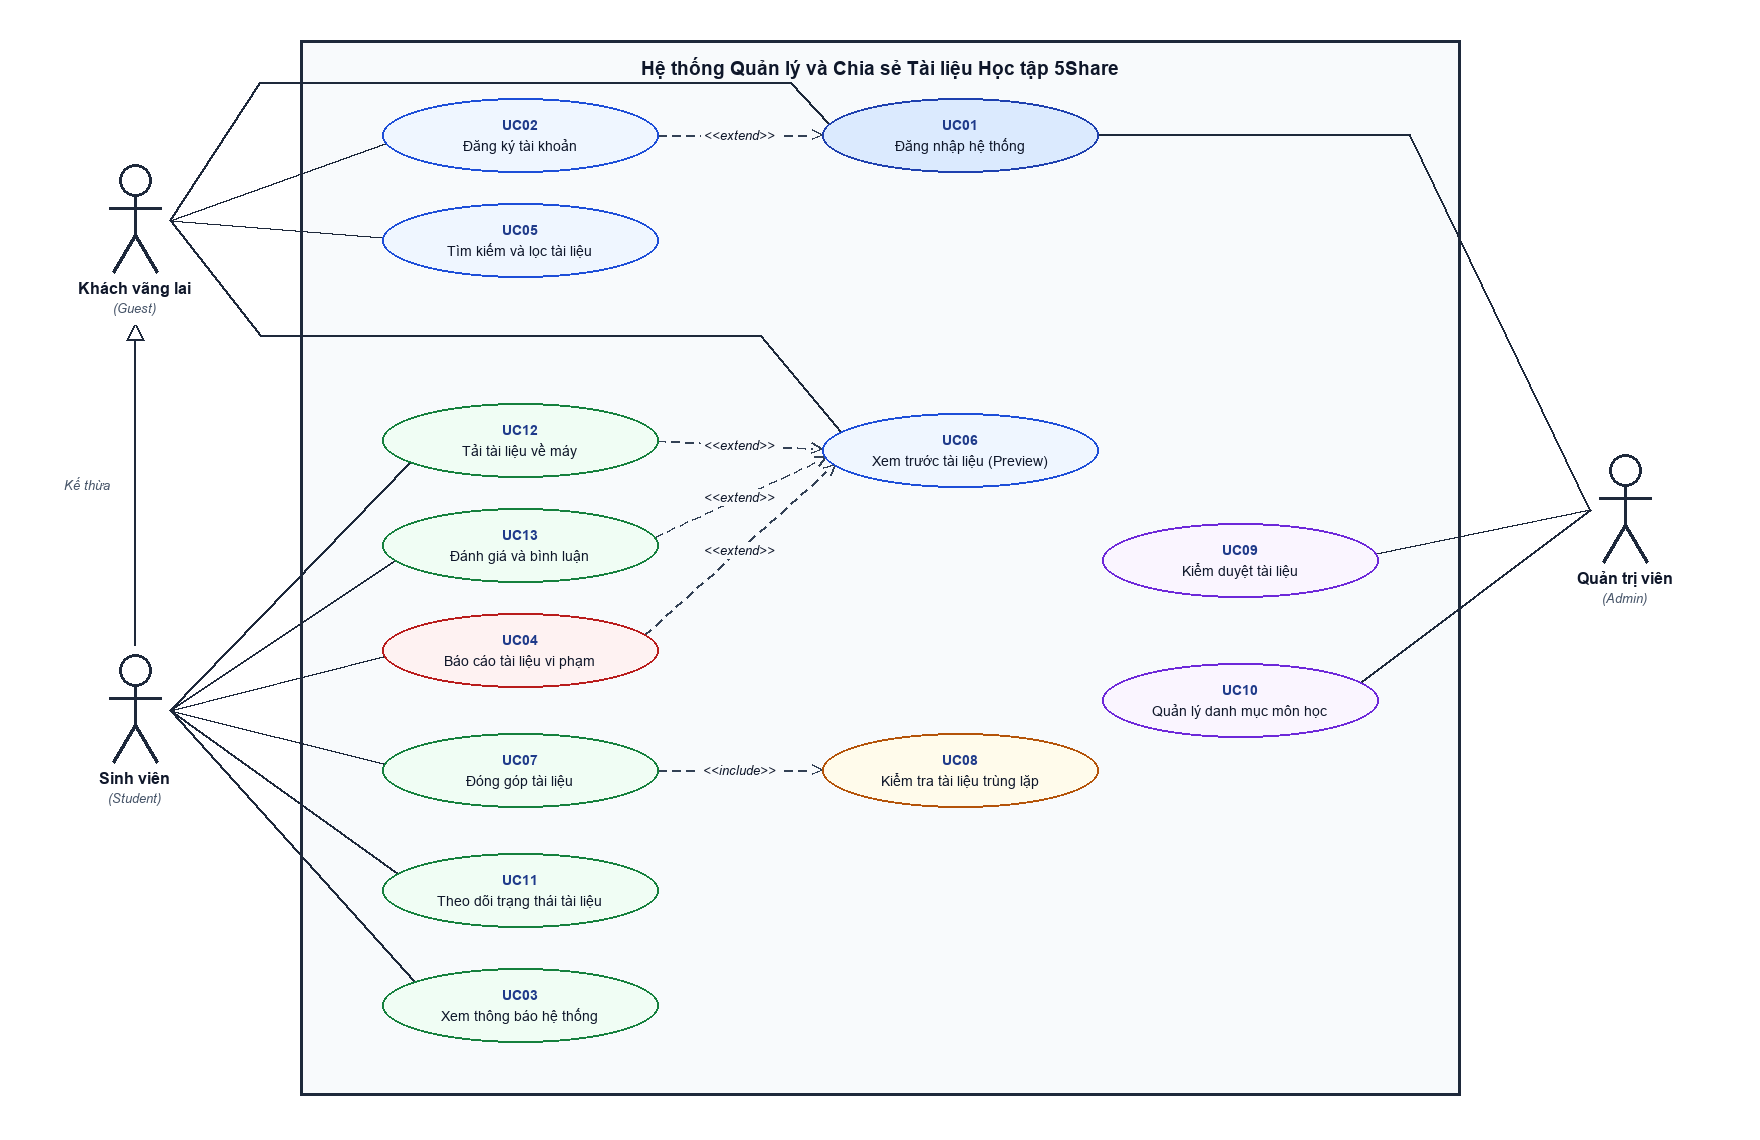
\includegraphics[width=0.98\textwidth]{chuong2/images/so_do_use_case_tong_quan.png}%
}{%
    \fbox{\parbox{0.95\textwidth}{\centering \vspace{3cm}\textbf{[Hình 2.1: Biểu đồ Use Case tổng quan của hệ thống 5Share]}\vspace{3cm}}}%
}
\caption{Biểu đồ Use Case tổng quan của hệ thống 5Share}
\label{fig:uc_tong_quan}
\end{figure}

\subsubsection{2.2.2. Biểu đồ Use Case phân rã cụm chức năng xác thực}
Để làm rõ các luồng mở rộng và cơ chế kiểm tra phân quyền tự động trong quá trình xác thực người dùng, ca sử dụng \texttt{UC01} (Đăng nhập hệ thống) được phân rã chi tiết ở mức 2 như minh họa tại Hình~\ref{fig:uc01_phan_ra}. Trong đó, ca sử dụng đăng nhập luôn bao hàm (\texttt{<<include>>}) bước xác thực mã phiên JWT và phân quyền theo vai trò lưu trong cơ sở dữ liệu, đồng thời cho phép mở rộng (\texttt{<<extend>>}) sang đăng ký tài khoản mới (\texttt{UC02}), khôi phục mật khẩu hoặc đăng nhập nhanh qua giao thức Google OAuth 2.0.

\begin{figure}[H]
\centering
\IfFileExists{chuong2/images/so_do_uc01_dang_nhap.png}{%
    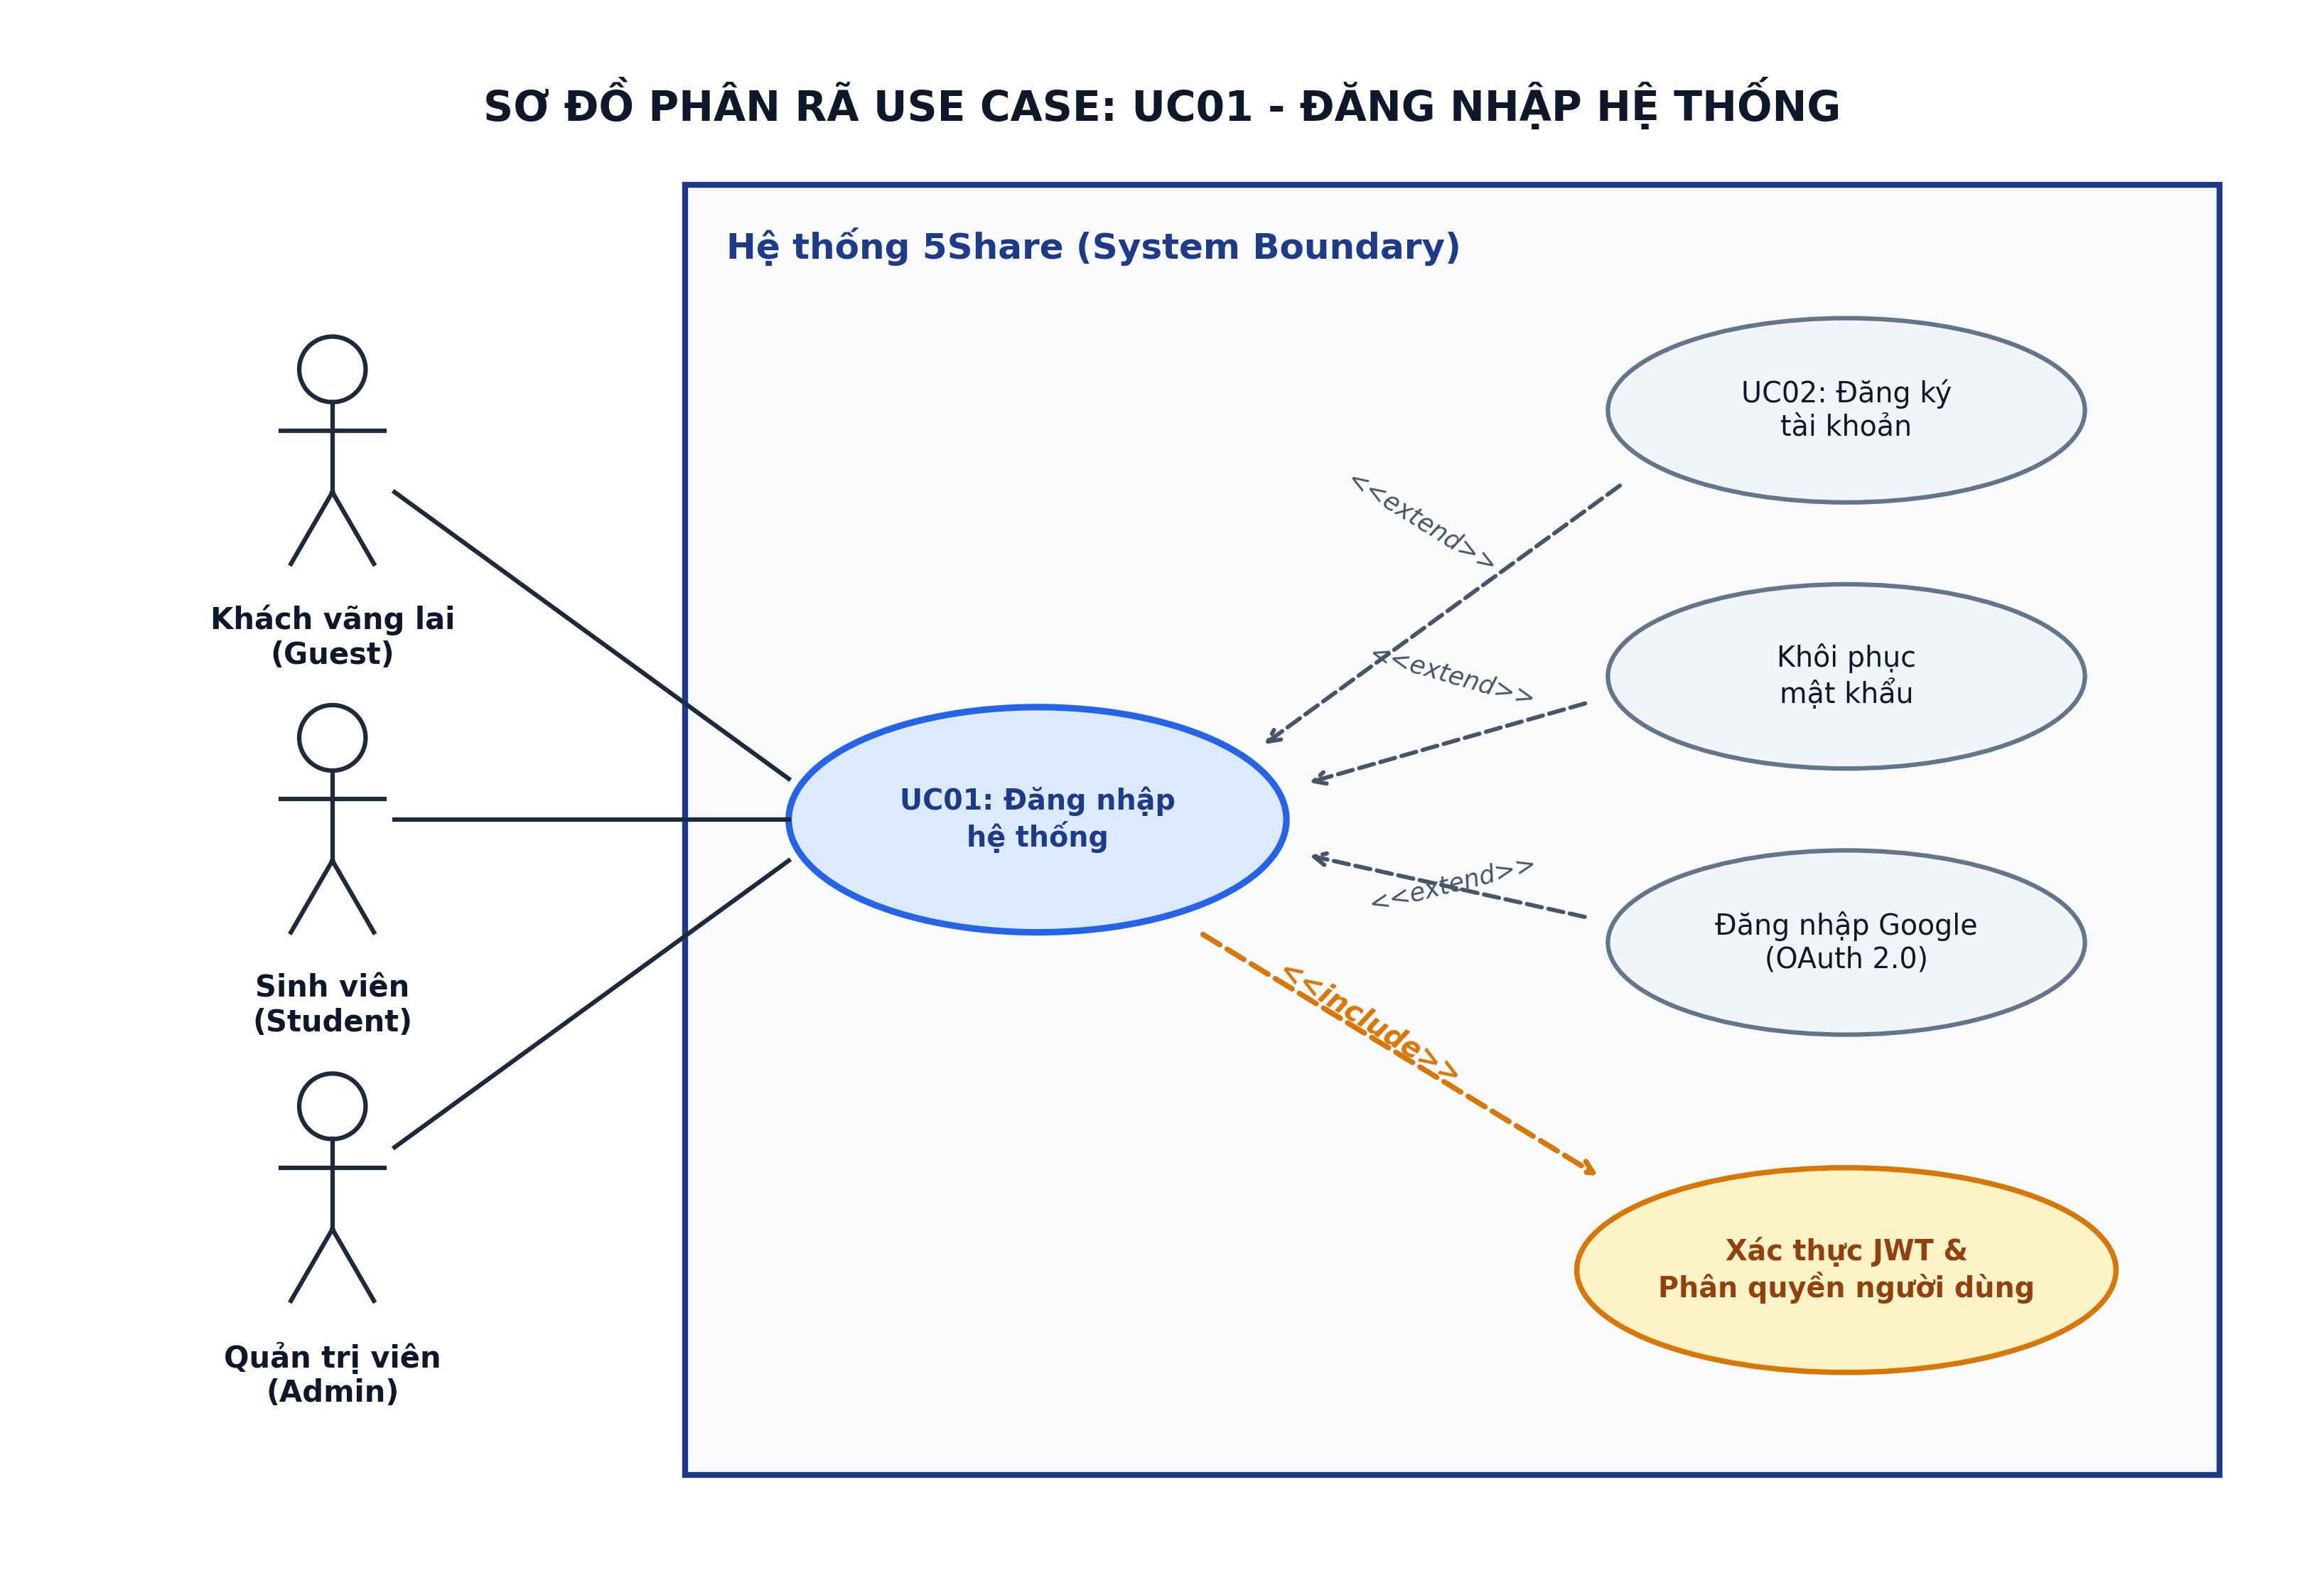
\includegraphics[width=0.92\textwidth]{chuong2/images/so_do_uc01_dang_nhap.png}%
}{%
    \fbox{\parbox{0.95\textwidth}{\centering \vspace{3cm}\textbf{[Hình 2.2: Biểu đồ Use Case phân rã chi tiết ca sử dụng Đăng nhập hệ thống (UC01)]}\vspace{3cm}}}%
}
\caption{Biểu đồ Use Case phân rã chi tiết ca sử dụng Đăng nhập hệ thống (UC01)}
\label{fig:uc01_phan_ra}
\end{figure}

\newpage
\subsection{2.3. Đặc tả chi tiết các ca sử dụng}

Mỗi ca sử dụng trong hệ thống 5Share được đặc tả chi tiết theo khung 09 trường thông tin tiêu chuẩn, bao gồm: Mục (Mã và Tên ca sử dụng), Actor (Tác nhân), Mô tả, Pre-conditions (Điều kiện tiên quyết), Action steps (Luồng sự kiện chính), Extension points (Các điểm mở rộng / Luồng rẽ nhánh), Exceptions (Các ngoại lệ / Xử lý lỗi), Post-conditions (Hậu điều kiện) và Yêu cầu liên quan (Truy vết yêu cầu).

\subsubsection{2.3.1. Nhóm ca sử dụng Xác thực và Quản lý tài khoản (UC01, UC02)}

\begin{table}[H]
\centering
\footnotesize\linespread{1.05}\selectfont
\setlength{\tabcolsep}{5pt}
\renewcommand{\arraystretch}{1.12}
\begin{tabularx}{\textwidth}{|p{3.5cm}|X|}
\hline
\rowcolor[HTML]{EAEAEA}
\textbf{Trường thông tin} & \textbf{Nội dung đặc tả chi tiết} \\
\hline
\textbf{Mục} & \textbf{UC01 -- Đăng nhập hệ thống} \\
\hline
\textbf{Actor} & Khách vãng lai, Sinh viên, Quản trị viên (Admin) \\
\hline
\textbf{Mô tả} & Người dùng xác thực danh tính bằng Email và Mật khẩu (hoặc Google) để đăng nhập vào hệ thống 5Share, nhận phiên làm việc và quyền hạn tương ứng. \\
\hline
\textbf{Pre-conditions} & Người dùng đã có tài khoản hợp lệ trên hệ thống; máy chủ và cơ sở dữ liệu hoạt động bình thường. \\
\hline
\textbf{Action steps} & 1. Người dùng nhấn vào nút ``Đăng nhập'' trên thanh điều hướng (Header).\newline 2. Hệ thống hiển thị cửa sổ (Modal) yêu cầu nhập Email và Mật khẩu.\newline 3. Người dùng nhập Email, Mật khẩu và nhấn nút ``Đăng nhập''.\newline 4. Hệ thống kiểm tra hợp lệ dữ liệu đầu vào (không để trống, đúng định dạng email).\newline 5. Hệ thống kiểm tra thông tin tài khoản trong cơ sở dữ liệu và đối chiếu mật khẩu đã băm (\texttt{bcrypt}).\newline 6. Hệ thống cấp mã phiên làm việc (JWT Token) chứa thông tin vai trò, hiển thị thông báo thành công và chuyển giao diện sang trạng thái đã đăng nhập. \\
\hline
\textbf{Extension points} & 2a. Chưa có tài khoản: Người dùng bấm ``Đăng ký ngay'' $\rightarrow$ Chuyển sang ca sử dụng \texttt{UC02} (Đăng ký tài khoản).\newline 3a. Quên mật khẩu: Người dùng bấm ``Quên mật khẩu'' $\rightarrow$ Nhập email để nhận liên kết đặt lại mật khẩu.\newline 3b. Đăng nhập Google: Người dùng chọn ``Đăng nhập với Google'' $\rightarrow$ Xác thực qua giao thức Google OAuth 2.0.\newline 3c. Hủy đăng nhập: Người dùng bấm nút đóng (X) $\rightarrow$ Đóng cửa sổ và giữ nguyên trang hiện tại. \\
\hline
\textbf{Exceptions} & E1 -- Bỏ trống thông tin: Chưa nhập email hoặc mật khẩu $\rightarrow$ Hệ thống cảnh báo: ``Vui lòng nhập đầy đủ Email và Mật khẩu''.\newline E2 -- Sai thông tin xác thực: Email hoặc mật khẩu không đúng $\rightarrow$ Hệ thống báo lỗi: ``Email hoặc mật khẩu không chính xác''.\newline E3 -- Tài khoản bị khóa: Tài khoản bị khóa do vi phạm quy định $\rightarrow$ Hệ thống báo: ``Tài khoản của bạn đã bị khóa, vui lòng liên hệ Quản trị viên''.\newline E4 -- Lỗi kết nối: Mất kết nối mạng hoặc gián đoạn máy chủ $\rightarrow$ Hệ thống báo: ``Không thể kết nối đến máy chủ, vui lòng thử lại sau''. \\
\hline
\textbf{Post-conditions} & Đăng nhập thành công; phiên làm việc được kích hoạt; thanh điều hướng hiển thị tên và ảnh đại diện; mở khóa quyền hạn tương ứng với vai trò (Sinh viên hoặc Quản trị viên). \\
\hline
\textbf{Yêu cầu liên quan} & \texttt{G5-FR03}; NFR: thời gian phản hồi xác thực $<$ 1 giây, mật khẩu đối chiếu qua hàm băm \texttt{bcrypt}. \\
\hline
\end{tabularx}
\caption{Đặc tả ca sử dụng UC01 -- Đăng nhập hệ thống}
\label{tab:uc01}
\end{table}


\begin{table}[H]
\centering
\footnotesize\linespread{1.05}\selectfont
\setlength{\tabcolsep}{5pt}
\renewcommand{\arraystretch}{1.12}
\begin{tabularx}{\textwidth}{|p{3.5cm}|X|}
\hline
\rowcolor[HTML]{EAEAEA}
\textbf{Trường thông tin} & \textbf{Nội dung đặc tả chi tiết} \\
\hline
\textbf{Mục} & \textbf{UC02 -- Đăng ký tài khoản} \\
\hline
\textbf{Actor} & Khách vãng lai \\
\hline
\textbf{Mô tả} & Khách vãng lai tạo tài khoản thành viên mới trên hệ thống 5Share bằng địa chỉ email hợp lệ để sử dụng các quyền đọc toàn văn, tải học liệu và đóng góp tài liệu. \\
\hline
\textbf{Pre-conditions} & Người dùng chưa đăng nhập; địa chỉ email đăng ký chưa từng tồn tại trong bảng \texttt{users} của cơ sở dữ liệu. \\
\hline
\textbf{Action steps} & 1. Người dùng nhấn nút ``Đăng ký'' trên thanh điều hướng hoặc chọn ``Đăng ký ngay'' từ cửa sổ đăng nhập (\texttt{UC01}).\newline 2. Hệ thống hiển thị biểu mẫu đăng ký gồm: Họ và tên, Địa chỉ Email, Mật khẩu và Xác nhận mật khẩu.\newline 3. Người dùng điền đầy đủ thông tin và nhấn nút ``Tạo tài khoản''.\newline 4. Hệ thống kiểm tra tính hợp lệ của dữ liệu (định dạng email, độ dài mật khẩu tối thiểu 8 ký tự, mật khẩu xác nhận trùng khớp).\newline 5. Hệ thống kiểm tra địa chỉ email chưa bị trùng lặp trong cơ sở dữ liệu.\newline 6. Hệ thống mã hóa mật khẩu bằng thuật toán \texttt{bcrypt}, tạo bản ghi người dùng mới với vai trò mặc định là Sinh viên (\texttt{USER}) và thông báo đăng ký thành công. \\
\hline
\textbf{Extension points} & 2a. Đã có tài khoản: Người dùng nhấn ``Đăng nhập ngay'' $\rightarrow$ Hệ thống chuyển về cửa sổ đăng nhập (\texttt{UC01}).\newline 3a. Hủy thao tác: Người dùng đóng biểu mẫu đăng ký $\rightarrow$ Hệ thống hủy dữ liệu đang nhập và quay lại màn hình trước đó. \\
\hline
\textbf{Exceptions} & E1 -- Dữ liệu không hợp lệ: Bỏ trống trường bắt buộc, email sai định dạng hoặc mật khẩu dưới 8 ký tự $\rightarrow$ Hệ thống hiển thị thông báo lỗi cụ thể dưới từng ô nhập.\newline E2 -- Mật khẩu xác nhận không khớp: Ô xác nhận mật khẩu khác ô mật khẩu $\rightarrow$ Hệ thống báo: ``Mật khẩu xác nhận không trùng khớp''.\newline E3 -- Email đã tồn tại: Địa chỉ email đã được đăng ký trước đó $\rightarrow$ Hệ thống cảnh báo: ``Email này đã được sử dụng, vui lòng đăng nhập hoặc dùng email khác''. \\
\hline
\textbf{Post-conditions} & Bản ghi tài khoản mới được lưu trữ an toàn trong cơ sở dữ liệu với \texttt{role = 'USER'}; người dùng được chuyển sang trạng thái đăng nhập để khai thác học liệu. \\
\hline
\textbf{Yêu cầu liên quan} & \texttt{G5-FR03}; NFR: mật khẩu bắt buộc mã hóa một chiều bằng \texttt{bcrypt} trước khi lưu vào cơ sở dữ liệu. \\
\hline
\end{tabularx}
\caption{Đặc tả ca sử dụng UC02 -- Đăng ký tài khoản}
\label{tab:uc02}
\end{table}


\subsubsection{2.3.2. Nhóm ca sử dụng Tra cứu, Xem trước và Tải học liệu (UC05, UC06, UC12)}

\begin{table}[H]
\centering
\footnotesize\linespread{1.05}\selectfont
\setlength{\tabcolsep}{5pt}
\renewcommand{\arraystretch}{1.12}
\begin{tabularx}{\textwidth}{|p{3.5cm}|X|}
\hline
\rowcolor[HTML]{EAEAEA}
\textbf{Trường thông tin} & \textbf{Nội dung đặc tả chi tiết} \\
\hline
\textbf{Mục} & \textbf{UC05 -- Tìm kiếm và lọc tài liệu} \\
\hline
\textbf{Actor} & Khách vãng lai, Sinh viên \\
\hline
\textbf{Mô tả} & Người dùng tra cứu học liệu trong kho công khai bằng từ khóa kết hợp các bộ lọc theo khối kiến thức, học kỳ, môn học và loại tài liệu (Kế hoạch bài dạy 5512, Đề thi, Bài giảng điện tử). \\
\hline
\textbf{Pre-conditions} & Cơ sở dữ liệu có các bản ghi môn học đang hoạt động và các tài liệu đã được phê duyệt (\texttt{status = 'APPROVED'}). \\
\hline
\textbf{Action steps} & 1. Người dùng nhập từ khóa vào thanh tìm kiếm hoặc chọn các tiêu chí lọc (Khối kiến thức, Học kỳ, Môn học, Loại tài liệu, Thứ tự sắp xếp).\newline 2. Người dùng nhấn nút ``Tìm kiếm'' hoặc thay đổi giá trị trên bộ lọc động.\newline 3. Hệ thống thực thi truy vấn tìm kiếm toàn văn (Full-Text Search) trên tiêu đề và mô tả tài liệu, đồng thời áp dụng điều kiện lọc chỉ lấy tài liệu có \texttt{status = 'APPROVED'}.\newline 4. Hệ thống phân trang kết quả (12 tài liệu/trang) và trả về danh sách các thẻ tài liệu khớp điều kiện kèm tổng số kết quả tìm thấy.\newline 5. Người dùng xem danh sách kết quả và nhấn vào một tài liệu để chuyển sang xem chi tiết (\texttt{UC06}). \\
\hline
\textbf{Extension points} & 1a. Xem theo cây danh mục chương trình đào tạo: Người dùng chọn trực tiếp một môn học trên thanh danh mục $\rightarrow$ Hệ thống liệt kê toàn bộ tài liệu đã duyệt của môn học đó.\newline 4a. Đổi tiêu chí sắp xếp: Người dùng chọn sắp xếp theo ``Mới nhất'', ``Tải nhiều nhất'' hoặc ``Đánh giá cao nhất'' $\rightarrow$ Hệ thống cập nhật lại thứ tự hiển thị danh sách. \\
\hline
\textbf{Exceptions} & E1 -- Không tìm thấy kết quả: Không có tài liệu nào khớp từ khóa và bộ lọc $\rightarrow$ Hệ thống hiển thị thông báo: ``Không tìm thấy học liệu phù hợp với tiêu chí tra cứu'' kèm nút ``Xóa bộ lọc''.\newline E2 -- Từ khóa chỉ chứa ký tự đặc biệt rỗng: Hệ thống tự động loại bỏ ký tự thừa và giữ nguyên danh sách học liệu công khai mặc định. \\
\hline
\textbf{Post-conditions} & Danh sách học liệu công khai thỏa mãn tiêu chí tìm kiếm và bộ lọc được hiển thị chính xác trên giao diện người dùng. \\
\hline
\textbf{Yêu cầu liên quan} & \texttt{G5-FR01} (liên kết \texttt{G5-FR08}); NFR: thời gian phản hồi truy vấn tìm kiếm và lọc $<$ 2 giây, hỗ trợ tiếng Việt có dấu và không dấu. \\
\hline
\end{tabularx}
\caption{Đặc tả ca sử dụng UC05 -- Tìm kiếm và lọc tài liệu}
\label{tab:uc05}
\end{table}


\begin{table}[H]
\centering
\footnotesize\linespread{1.05}\selectfont
\setlength{\tabcolsep}{5pt}
\renewcommand{\arraystretch}{1.12}
\begin{tabularx}{\textwidth}{|p{3.5cm}|X|}
\hline
\rowcolor[HTML]{EAEAEA}
\textbf{Trường thông tin} & \textbf{Nội dung đặc tả chi tiết} \\
\hline
\textbf{Mục} & \textbf{UC06 -- Xem trước tài liệu} \\
\hline
\textbf{Actor} & Khách vãng lai, Sinh viên \\
\hline
\textbf{Mô tả} & Người dùng đọc trực tiếp nội dung tệp tin PDF ngay trên trình duyệt web thông qua trình đọc tích hợp, với cơ chế giới hạn 3 trang đầu đối với Khách vãng lai và hiển thị toàn văn đối với Sinh viên đã đăng nhập. \\
\hline
\textbf{Pre-conditions} & Tài liệu được chọn đang ở trạng thái công khai (\texttt{status = 'APPROVED'}) hoặc người xem là Quản trị viên / Tác giả của tài liệu. \\
\hline
\textbf{Action steps} & 1. Người dùng nhấn vào tên hoặc thẻ của một tài liệu từ danh sách kết quả tra cứu (\texttt{UC05}).\newline 2. Hệ thống chuyển hướng đến trang chi tiết tài liệu, truy xuất thông tin metadata, điểm đánh giá trung bình và danh sách bình luận.\newline 3. Hệ thống kiểm tra trạng thái phiên xác thực (JWT Token) của người dùng hiện tại.\newline 4. Nếu người dùng đã đăng nhập (Sinh viên), hệ thống tải luồng dữ liệu PDF và hiển thị toàn bộ số trang của tài liệu trên khung đọc trực tuyến (Full PDF Preview), đồng thời tăng bộ đếm lượt xem thêm 1.\newline 5. Người dùng cuộn trang, phóng to/thu nhỏ để đọc nội dung học liệu trực tiếp trên trình duyệt. \\
\hline
\textbf{Extension points} & 3a. Người dùng là Khách vãng lai (chưa đăng nhập): Hệ thống chỉ cho phép trình đọc PDF hiển thị tối đa 3 trang đầu tiên của tài liệu và hiển thị thông báo ở cuối trang 3: ``Vui lòng đăng nhập để đọc toàn văn và tải tài liệu''.\newline 5a. Tải tài liệu hoặc Lưu vào tủ cá nhân: Người dùng nhấn nút ``Tải về'' hoặc ``Lưu vào tủ'' $\rightarrow$ Mở rộng sang ca sử dụng \texttt{UC12} (nếu là Khách vãng lai thì hệ thống bật cửa sổ yêu cầu đăng nhập \texttt{UC01}).\newline 5b. Đánh giá hoặc Bình luận: Sinh viên nhấn chọn số sao hoặc viết bình luận dưới tài liệu $\rightarrow$ Mở rộng sang ca sử dụng \texttt{UC13}.\newline 5c. Báo cáo sai phạm: Sinh viên nhấn nút ``Báo cáo vi phạm'' $\rightarrow$ Mở rộng sang ca sử dụng \texttt{UC04}. \\
\hline
\textbf{Exceptions} & E1 -- Lỗi tải tệp PDF từ đám mây: Đường dẫn lưu trữ đám mây bị gián đoạn $\rightarrow$ Hệ thống hiển thị thông báo: ``Không thể tải bản xem trước lúc này, vui lòng thử lại sau''.\newline E2 -- Tài liệu vừa bị ẩn hoặc xóa: Tài liệu không còn ở trạng thái hợp lệ $\rightarrow$ Hệ thống điều hướng về trang thông báo tài liệu không tồn tại. \\
\hline
\textbf{Post-conditions} & Nội dung tài liệu được hiển thị đúng phân quyền (3 trang đầu cho Khách vãng lai, toàn văn cho Sinh viên); số lượt xem (\texttt{view\_count}) của tài liệu được cập nhật. \\
\hline
\textbf{Yêu cầu liên quan} & \texttt{G5-FR02}, \texttt{G5-FR03}; NFR: thời gian hiển thị 3 trang đầu tiên trên trình duyệt $<$ 2,5 giây; tích hợp bộ font chuẩn hiển thị tiếng Việt. \\
\hline
\end{tabularx}
\caption{Đặc tả ca sử dụng UC06 -- Xem trước tài liệu}
\label{tab:uc06}
\end{table}


\begin{table}[H]
\centering
\footnotesize\linespread{1.05}\selectfont
\setlength{\tabcolsep}{5pt}
\renewcommand{\arraystretch}{1.12}
\begin{tabularx}{\textwidth}{|p{3.5cm}|X|}
\hline
\rowcolor[HTML]{EAEAEA}
\textbf{Trường thông tin} & \textbf{Nội dung đặc tả chi tiết} \\
\hline
\textbf{Mục} & \textbf{UC12 -- Tải tài liệu về máy} \\
\hline
\textbf{Actor} & Sinh viên \\
\hline
\textbf{Mô tả} & Sinh viên đã đăng nhập thực hiện tải tệp tin PDF gốc về thiết bị cá nhân để phục vụ học tập hoặc đánh dấu lưu tài liệu vào Tủ tài liệu cá nhân (Bookmark). \\
\hline
\textbf{Pre-conditions} & Người dùng đã đăng nhập hệ thống với vai trò Sinh viên (hoặc Quản trị viên); tài liệu đang ở trạng thái đã duyệt (\texttt{status = 'APPROVED'}). \\
\hline
\textbf{Action steps} & 1. Tại trang xem chi tiết tài liệu (\texttt{UC06}), sinh viên nhấn vào nút ``Tải xuống (.pdf)''.\newline 2. Hệ thống xác thực mã phiên JWT của người dùng nhằm bảo đảm yêu cầu tải đến từ thành viên đã đăng nhập.\newline 3. Hệ thống ghi nhận bản ghi lịch sử tải xuống, tăng chỉ số lượt tải (\texttt{download\_count}) của tài liệu thêm 1 đơn vị trong cơ sở dữ liệu.\newline 4. Hệ thống cấp đường dẫn tệp tin gốc từ máy chủ lưu trữ đám mây (Cloudinary) và kích hoạt trình duyệt tải tệp \texttt{.pdf} về thiết bị của sinh viên. \\
\hline
\textbf{Extension points} & 1a. Khách vãng lai bấm nút ``Tải xuống'' hoặc ``Lưu vào tủ'': Hệ thống chặn API tải tệp gốc và tự động mở cửa sổ yêu cầu xác thực đăng nhập (\texttt{UC01}).\newline 1b. Đánh dấu lưu vào Tủ tài liệu cá nhân (Bookmark): Sinh viên nhấn biểu tượng ``Lưu vào tủ'' $\rightarrow$ Hệ thống thêm (hoặc gỡ) bản ghi trong bảng \texttt{bookmarks}, đổi màu biểu tượng đánh dấu và cập nhật danh sách trong mục ``Tủ tài liệu cá nhân''. \\
\hline
\textbf{Exceptions} & E1 -- Phiên đăng nhập hết hạn: Mã JWT hết hiệu lực tại thời điểm bấm tải $\rightarrow$ Hệ thống thông báo phiên làm việc đã hết hạn và yêu cầu đăng nhập lại (\texttt{UC01}).\newline E2 -- Gián đoạn kết nối máy chủ lưu trữ: Không lấy được luồng tệp từ đám mây $\rightarrow$ Hệ thống báo lỗi: ``Quá trình tải tệp bị gián đoạn, vui lòng thử lại'' và không cộng lùi lượt tải ảo. \\
\hline
\textbf{Post-conditions} & Tệp tin PDF gốc được lưu về thiết bị cá nhân của sinh viên; bộ đếm lượt tải (\texttt{download\_count}) tăng thêm 1 (hoặc trạng thái Bookmark được cập nhật trong Tủ tài liệu cá nhân). \\
\hline
\textbf{Yêu cầu liên quan} & \texttt{G5-FR04} (liên kết \texttt{G5-FR02}); NFR: che giấu đường dẫn lưu trữ gốc, chặn truy cập tải trực tiếp từ người dùng chưa xác thực. \\
\hline
\end{tabularx}
\caption{Đặc tả ca sử dụng UC12 -- Tải tài liệu về máy}
\label{tab:uc12}
\end{table}


\subsubsection{2.3.3. Nhóm ca sử dụng Đóng góp và Chống trùng lặp học liệu (UC07, UC08)}

\begin{table}[H]
\centering
\footnotesize\linespread{1.05}\selectfont
\setlength{\tabcolsep}{5pt}
\renewcommand{\arraystretch}{1.12}
\begin{tabularx}{\textwidth}{|p{3.5cm}|X|}
\hline
\rowcolor[HTML]{EAEAEA}
\textbf{Trường thông tin} & \textbf{Nội dung đặc tả chi tiết} \\
\hline
\textbf{Mục} & \textbf{UC07 -- Đóng góp tài liệu} \\
\hline
\textbf{Actor} & Sinh viên \\
\hline
\textbf{Mô tả} & Sinh viên đã đăng nhập tải tệp tin học liệu (.pdf) kèm đầy đủ thông tin đặc tả (Metadata) lên hệ thống để chia sẻ cho cộng đồng sau khi vượt qua bước kiểm tra tự động và chờ Quản trị viên thẩm định. \\
\hline
\textbf{Pre-conditions} & Người dùng đã đăng nhập với vai trò Sinh viên; danh mục môn học và loại tài liệu đã được khởi tạo trong cơ sở dữ liệu. \\
\hline
\textbf{Action steps} & 1. Sinh viên nhấn nút ``Đóng góp tài liệu'' trên thanh điều hướng để mở biểu mẫu tải lên.\newline 2. Sinh viên chọn tệp tin (\texttt{.pdf}) từ thiết bị cá nhân và điền các trường Metadata bắt buộc: Tiêu đề tài liệu (tối thiểu 10 ký tự), Môn học, Loại tài liệu (Kế hoạch bài dạy 5512 / Đề thi / Bài giảng) và Mô tả tóm tắt.\newline 3. Sinh viên nhấn nút ``Gửi đóng góp''.\newline 4. Hệ thống kiểm tra hợp lệ các trường Metadata và kiểm tra kỹ thuật tệp tin: phần mở rộng \texttt{.pdf}, dung lượng $\le$ 25MB và chuỗi chữ ký nhị phân đầu tệp (Magic Bytes \texttt{\%PDF-}).\newline 5. Hệ thống tự động gọi ca sử dụng bao hàm \texttt{UC08} (Kiểm tra tài liệu trùng lặp) để băm \texttt{SHA-256} và đối chiếu trùng lặp.\newline 6. Khi tệp tin hợp lệ và không trùng lặp, hệ thống tải tệp lên dịch vụ đám mây Cloudinary, lưu bản ghi mới vào bảng \texttt{documents} với trạng thái mặc định \texttt{status = 'PENDING'} và hiển thị thông báo đóng góp thành công. \\
\hline
\textbf{Extension points} & 2a. Thay đổi tệp tin trước khi gửi: Sinh viên nhấn ``Chọn lại tệp'' $\rightarrow$ Hệ thống xóa tệp tạm trên biểu mẫu để sinh viên chọn tệp PDF khác.\newline 3a. Hủy đóng góp: Sinh viên nhấn nút ``Hủy'' $\rightarrow$ Hệ thống xóa dữ liệu trên biểu mẫu và quay về trang trước. \\
\hline
\textbf{Exceptions} & E1 -- Thiếu thông tin Metadata: Bỏ trống trường bắt buộc hoặc tiêu đề dưới 10 ký tự $\rightarrow$ Hệ thống cảnh báo và yêu cầu bổ sung.\newline E2 -- Sai định dạng hoặc giả mạo tệp PDF: Tệp không phải đuôi \texttt{.pdf} hoặc không chứa Magic Bytes \texttt{\%PDF-} $\rightarrow$ Hệ thống chặn tiếp nhận và báo: ``Chỉ chấp nhận tệp tin chuẩn định dạng PDF''.\newline E3 -- Vượt quá dung lượng cho phép: Tệp tin lớn hơn 25MB $\rightarrow$ Hệ thống báo lỗi: ``Dung lượng tệp vượt quá giới hạn tối đa 25MB''.\newline E4 -- Phát hiện tệp tin trùng lặp (từ \texttt{UC08}): Mã băm \texttt{SHA-256} đã tồn tại $\rightarrow$ Hệ thống từ chối lưu trữ và thông báo tài liệu đã có trên hệ thống. \\
\hline
\textbf{Post-conditions} & Tệp PDF được lưu trữ trên đám mây; bản ghi tài liệu mới được khởi tạo với \texttt{status = 'PENDING'} (ẩn hoàn toàn khỏi kho công khai, chỉ hiển thị trong mục theo dõi của tác giả và hàng đợi kiểm duyệt của Quản trị viên). \\
\hline
\textbf{Yêu cầu liên quan} & \texttt{G5-FR05}, \texttt{G5-FR06}, \texttt{G5-FR13}; NFR: kiểm tra dung lượng $\le$ 25MB và chữ ký nhị phân Magic Bytes \texttt{\%PDF-}. \\
\hline
\end{tabularx}
\caption{Đặc tả ca sử dụng UC07 -- Đóng góp tài liệu}
\label{tab:uc07}
\end{table}


\begin{table}[H]
\centering
\footnotesize\linespread{1.05}\selectfont
\setlength{\tabcolsep}{5pt}
\renewcommand{\arraystretch}{1.12}
\begin{tabularx}{\textwidth}{|p{3.5cm}|X|}
\hline
\rowcolor[HTML]{EAEAEA}
\textbf{Trường thông tin} & \textbf{Nội dung đặc tả chi tiết} \\
\hline
\textbf{Mục} & \textbf{UC08 -- Kiểm tra tài liệu trùng lặp} \\
\hline
\textbf{Actor} & Hệ thống tự động (được kích hoạt qua quan hệ \texttt{<<include>>} từ \texttt{UC07}) \\
\hline
\textbf{Mô tả} & Hệ thống tự động tính toán mã băm mật mã học \texttt{SHA-256} từ nội dung nhị phân của tệp PDF tải lên và đối chiếu với cơ sở dữ liệu nhằm ngăn chặn triệt để việc đăng tải lại các tệp tin đã tồn tại. \\
\hline
\textbf{Pre-conditions} & Ca sử dụng \texttt{UC07} đã kiểm tra tệp tin thỏa mãn định dạng PDF, chữ ký Magic Bytes \texttt{\%PDF-} và dung lượng $\le$ 25MB. \\
\hline
\textbf{Action steps} & 1. Hệ thống tiếp nhận luồng dữ liệu nhị phân (binary buffer) của tệp tin PDF từ ca sử dụng \texttt{UC07}.\newline 2. Hệ thống áp dụng thuật toán băm \texttt{SHA-256} để sinh chuỗi mã băm duy nhất có độ dài 64 ký tự hệ thập lục phân (hexadecimal).\newline 3. Hệ thống thực thi câu lệnh truy vấn đối chiếu chuỗi mã băm vừa sinh với cột \texttt{file\_hash} trong bảng \texttt{documents} của cơ sở dữ liệu.\newline 4. Nếu không tìm thấy bản ghi trùng khớp, hệ thống xác nhận tệp tin là duy nhất, gắn giá trị \texttt{file\_hash} vào bản ghi mới và trả kết quả hợp lệ về \texttt{UC07} để tiếp tục tải lên đám mây. \\
\hline
\textbf{Extension points} & Không có điểm mở rộng (đây là quy trình kiểm tra tự động bắt buộc ở tầng máy chủ). \\
\hline
\textbf{Exceptions} & E1 -- Phát hiện mã băm trùng khớp: Cột \texttt{file\_hash} trong bảng \texttt{documents} đã tồn tại chuỗi mã băm tương tự $\rightarrow$ Hệ thống lập tức hủy luồng tải lên Cloudinary, giải phóng bộ nhớ tạm và trả thông báo cảnh báo về giao diện \texttt{UC07}: ``Tài liệu này đã tồn tại trên hệ thống (trùng nội dung tệp tin), vui lòng không đăng tải lặp lại''.\newline E2 -- Lỗi đọc luồng nhị phân: Tệp tin bị hỏng cấu trúc trong quá trình truyền tải $\rightarrow$ Hệ thống hủy thao tác và báo lỗi tệp tin bị hỏng. \\
\hline
\textbf{Post-conditions} & Hệ thống xác định chính xác tính duy nhất của tệp tin; mọi tệp tin trùng lặp nội dung nhị phân đều bị chặn trước khi tiêu tốn dung lượng lưu trữ đám mây. \\
\hline
\textbf{Yêu cầu liên quan} & \texttt{G5-FR13} (hỗ trợ \texttt{G5-FR05}); NFR: thời gian tính toán \texttt{SHA-256} và truy vấn đối chiếu chỉ mục $<$ 500ms cho tệp 25MB. \\
\hline
\end{tabularx}
\caption{Đặc tả ca sử dụng UC08 -- Kiểm tra tài liệu trùng lặp}
\label{tab:uc08}
\end{table}


\subsubsection{2.3.4. Nhóm ca sử dụng Tương tác học thuật và Thông báo (UC03, UC04, UC13)}

\begin{table}[H]
\centering
\footnotesize\linespread{1.05}\selectfont
\setlength{\tabcolsep}{5pt}
\renewcommand{\arraystretch}{1.12}
\begin{tabularx}{\textwidth}{|p{3.5cm}|X|}
\hline
\rowcolor[HTML]{EAEAEA}
\textbf{Trường thông tin} & \textbf{Nội dung đặc tả chi tiết} \\
\hline
\textbf{Mục} & \textbf{UC03 -- Xem thông báo hệ thống} \\
\hline
\textbf{Actor} & Sinh viên \\
\hline
\textbf{Mô tả} & Sinh viên nhận và xem các thông báo tự động từ hệ thống trên biểu tượng chuông thông báo khi tài liệu đóng góp được phê duyệt, bị từ chối kèm lý do, hoặc khi có bình luận trao đổi mới. \\
\hline
\textbf{Pre-conditions} & Sinh viên đã đăng nhập vào hệ thống; có sự kiện nghiệp vụ phát sinh bản ghi thông báo mới trong bảng \texttt{notifications}. \\
\hline
\textbf{Action steps} & 1. Khi phát sinh sự kiện (Quản trị viên duyệt/từ chối tài liệu tại \texttt{UC09} hoặc có bình luận mới tại \texttt{UC13}), hệ thống tự động khởi tạo bản ghi thông báo gắn với \texttt{user\_id} của người nhận.\newline 2. Giao diện thanh điều hướng của sinh viên hiển thị biểu tượng Chuông kèm nhãn số lượng thông báo chưa đọc (unread badge).\newline 3. Sinh viên nhấn vào biểu tượng Chuông thông báo.\newline 4. Hệ thống hiển thị danh sách thả xuống (Dropdown) liệt kê các thông báo theo thứ tự thời gian từ mới nhất đến cũ nhất.\newline 5. Sinh viên nhấn vào một thông báo cụ thể $\rightarrow$ Hệ thống cập nhật trạng thái thông báo thành ``Đã đọc'' (\texttt{is\_read = true}), giảm số đếm chưa đọc và điều hướng đến trang tài liệu liên quan. \\
\hline
\textbf{Extension points} & 4a. Đánh dấu tất cả là đã đọc: Sinh viên nhấn nút ``Đánh dấu đã đọc tất cả'' $\rightarrow$ Hệ thống cập nhật toàn bộ thông báo hiện có sang trạng thái đã đọc và ẩn nhãn số đếm màu đỏ. \\
\hline
\textbf{Exceptions} & E1 -- Chưa có thông báo nào: Bảng thông báo của người dùng đang trống $\rightarrow$ Khi nhấn vào chuông, hệ thống hiển thị trạng thái trống: ``Bạn chưa có thông báo mới nào''.\newline E2 -- Tài liệu liên kết đã bị xóa: Người dùng nhấn vào thông báo cũ của một tài liệu đã bị gỡ bỏ $\rightarrow$ Hệ thống hiển thị thông báo tài liệu không còn tồn tại. \\
\hline
\textbf{Post-conditions} & Sinh viên nắm bắt kịp thời kết quả kiểm duyệt (kèm lý do từ chối nếu có) và các phản hồi học thuật; trạng thái đã đọc của thông báo được đồng bộ trong cơ sở dữ liệu. \\
\hline
\textbf{Yêu cầu liên quan} & \texttt{G5-FR11} (liên kết \texttt{G5-FR07}); NFR: truy vấn danh sách thông báo phản hồi $<$ 500ms. \\
\hline
\end{tabularx}
\caption{Đặc tả ca sử dụng UC03 -- Xem thông báo hệ thống}
\label{tab:uc03}
\end{table}


\begin{table}[H]
\centering
\footnotesize\linespread{1.05}\selectfont
\setlength{\tabcolsep}{5pt}
\renewcommand{\arraystretch}{1.12}
\begin{tabularx}{\textwidth}{|p{3.5cm}|X|}
\hline
\rowcolor[HTML]{EAEAEA}
\textbf{Trường thông tin} & \textbf{Nội dung đặc tả chi tiết} \\
\hline
\textbf{Mục} & \textbf{UC04 -- Báo cáo tài liệu vi phạm} \\
\hline
\textbf{Actor} & Sinh viên \\
\hline
\textbf{Mô tả} & Sinh viên gửi báo cáo cảnh báo đến Quản trị viên khi phát hiện tài liệu đang lưu hành có nội dung sai lệch kiến thức, không đúng chuẩn Công văn 5512, lỗi hiển thị hoặc vi phạm bản quyền. \\
\hline
\textbf{Pre-conditions} & Người dùng đã đăng nhập với vai trò Sinh viên và đang ở trang xem chi tiết một tài liệu công khai (\texttt{UC06}). \\
\hline
\textbf{Action steps} & 1. Tại trang chi tiết tài liệu (\texttt{UC06}), sinh viên nhấn vào nút ``Báo cáo vi phạm''.\newline 2. Hệ thống hiển thị hộp thoại yêu cầu chọn nhóm lý do vi phạm (Sai kiến thức chuyên môn / Không đúng môn học / Vi phạm bản quyền / Tệp mờ nhòe, lỗi font) và ô nhập mô tả chi tiết.\newline 3. Sinh viên chọn lý do, nhập nội dung giải trình cụ thể và nhấn nút ``Gửi báo cáo''.\newline 4. Hệ thống kiểm tra dữ liệu hợp lệ và kiểm tra sinh viên chưa gửi báo cáo trùng lặp cho cùng tài liệu này.\newline 5. Hệ thống lưu bản ghi mới vào bảng \texttt{reports} với trạng thái \texttt{status = 'PENDING'} và hiển thị thông báo cảm ơn sinh viên đã đóng góp phản hồi. \\
\hline
\textbf{Extension points} & 3a. Hủy gửi báo cáo: Sinh viên nhấn nút ``Hủy'' hoặc đóng hộp thoại $\rightarrow$ Hệ thống hủy thao tác và giữ nguyên màn hình xem tài liệu. \\
\hline
\textbf{Exceptions} & E1 -- Chưa chọn hoặc nhập lý do: Sinh viên để trống nội dung báo cáo $\rightarrow$ Hệ thống cảnh báo: ``Vui lòng chọn lý do và mô tả chi tiết dấu hiệu vi phạm''.\newline E2 -- Báo cáo trùng lặp: Sinh viên đã gửi báo cáo cho tài liệu này trước đó và báo cáo đang chờ xử lý $\rightarrow$ Hệ thống thông báo: ``Báo cáo trước đó của bạn cho tài liệu này đang được Quản trị viên xem xét''. \\
\hline
\textbf{Post-conditions} & Bản ghi báo cáo vi phạm được lưu vào bảng \texttt{reports} với \texttt{status = 'PENDING'} và xuất hiện trong danh sách cần xử lý của Quản trị viên (\texttt{UC09}). \\
\hline
\textbf{Yêu cầu liên quan} & \texttt{G5-FR10}; NFR: chống gửi báo cáo rác lặp lại từ cùng một tài khoản trên một tài liệu. \\
\hline
\end{tabularx}
\caption{Đặc tả ca sử dụng UC04 -- Báo cáo tài liệu vi phạm}
\label{tab:uc04}
\end{table}


\begin{table}[H]
\centering
\footnotesize\linespread{1.05}\selectfont
\setlength{\tabcolsep}{5pt}
\renewcommand{\arraystretch}{1.12}
\begin{tabularx}{\textwidth}{|p{3.5cm}|X|}
\hline
\rowcolor[HTML]{EAEAEA}
\textbf{Trường thông tin} & \textbf{Nội dung đặc tả chi tiết} \\
\hline
\textbf{Mục} & \textbf{UC13 -- Đánh giá và bình luận tài liệu} \\
\hline
\textbf{Actor} & Sinh viên \\
\hline
\textbf{Mô tả} & Sinh viên đã đăng nhập thực hiện chấm điểm chất lượng học liệu theo thang 1--5 sao và đăng tải bình luận trao đổi học thuật dưới trang chi tiết tài liệu. \\
\hline
\textbf{Pre-conditions} & Người dùng đã đăng nhập với vai trò Sinh viên; tài liệu đang ở trạng thái công khai (\texttt{status = 'APPROVED'}). \\
\hline
\textbf{Action steps} & 1. Tại khu vực tương tác dưới trang chi tiết tài liệu (\texttt{UC06}), sinh viên chọn mức điểm từ 1 đến 5 sao và/hoặc nhập nội dung nhận xét vào khung bình luận.\newline 2. Sinh viên nhấn nút ``Gửi đánh giá / Bình luận''.\newline 3. Hệ thống kiểm tra quy tắc mỗi tài khoản chỉ giữ một kết quả chấm sao trên mỗi tài liệu (nếu đã chấm trước đó thì cập nhật lại số sao mới) và kiểm tra nội dung bình luận không rỗng.\newline 4. Hệ thống lưu điểm đánh giá và nội dung bình luận vào cơ sở dữ liệu, tự động tính toán lại điểm trung bình cộng \texttt{AVG(rating)} của tài liệu.\newline 5. Hệ thống cập nhật điểm sao trung bình và hiển thị bình luận mới kèm tên tác giả, thời gian đăng ngay dưới tài liệu. \\
\hline
\textbf{Extension points} & 1a. Chỉ chấm sao không kèm bình luận chữ (hoặc ngược lại): Hệ thống ghi nhận phần dữ liệu tương ứng và cập nhật giao diện tức thì.\newline 5a. Chỉnh sửa hoặc xóa bình luận cá nhân: Sinh viên nhấn ``Sửa'' hoặc ``Xóa'' trên bình luận của chính mình $\rightarrow$ Hệ thống cập nhật hoặc gỡ bỏ bình luận đó. \\
\hline
\textbf{Exceptions} & E1 -- Bình luận rỗng hoặc quá giới hạn ký tự: Nội dung chỉ có khoảng trắng hoặc vượt quá 1.000 ký tự $\rightarrow$ Hệ thống cảnh báo yêu cầu nhập nội dung hợp lệ.\newline E2 -- Khách vãng lai nhấn vào khu vực đánh giá/bình luận: Hệ thống hiển thị thông báo yêu cầu đăng nhập tài khoản (\texttt{UC01}). \\
\hline
\textbf{Post-conditions} & Điểm đánh giá trung bình của tài liệu và danh sách bình luận học thuật được cập nhật chính xác theo thời gian thực; tác giả tài liệu nhận được thông báo tương tác mới (\texttt{UC03}). \\
\hline
\textbf{Yêu cầu liên quan} & \texttt{G5-FR09}; NFR: ràng buộc duy nhất 1 lượt chấm sao/người dùng/tài liệu, cập nhật điểm trung bình tức thì. \\
\hline
\end{tabularx}
\caption{Đặc tả ca sử dụng UC13 -- Đánh giá và bình luận tài liệu}
\label{tab:uc13}
\end{table}


\subsubsection{2.3.5. Nhóm ca sử dụng Kiểm duyệt, Quản trị và Theo dõi tài liệu (UC09, UC10, UC11)}

\begin{table}[H]
\centering
\footnotesize\linespread{1.05}\selectfont
\setlength{\tabcolsep}{5pt}
\renewcommand{\arraystretch}{1.12}
\begin{tabularx}{\textwidth}{|p{3.5cm}|X|}
\hline
\rowcolor[HTML]{EAEAEA}
\textbf{Trường thông tin} & \textbf{Nội dung đặc tả chi tiết} \\
\hline
\textbf{Mục} & \textbf{UC09 -- Kiểm duyệt tài liệu} \\
\hline
\textbf{Actor} & Quản trị viên (Admin) \\
\hline
\textbf{Mô tả} & Quản trị viên thẩm định các tài liệu trong hàng đợi chờ duyệt (\texttt{PENDING}) theo 8 tiêu chí chuyên môn để quyết định Phê duyệt (\texttt{APPROVED}) hoặc Từ chối (\texttt{REJECTED}) kèm lý do, đồng thời xử lý các báo cáo tài liệu vi phạm. \\
\hline
\textbf{Pre-conditions} & Người dùng đã đăng nhập bằng tài khoản Quản trị viên; có tài liệu ở trạng thái \texttt{PENDING} hoặc có báo cáo vi phạm đang chờ xử lý. \\
\hline
\textbf{Action steps} & 1. Quản trị viên truy cập Phân hệ Quản trị và mở danh sách ``Hàng đợi chờ kiểm duyệt''.\newline 2. Hệ thống liệt kê các tài liệu có \texttt{status = 'PENDING'} kèm thông tin người đóng góp, môn học, loại tài liệu và thời gian tải lên.\newline 3. Quản trị viên chọn một tài liệu để mở trình đọc toàn văn (Full PDF Preview) và đối chiếu nội dung với tiêu chuẩn học thuật (cấu trúc 4 hoạt động Công văn 5512, tính chính xác, bản quyền, độ rõ nét).\newline 4. Nếu tài liệu đạt yêu cầu, Quản trị viên nhấn nút ``Phê duyệt (Approve)''.\newline 5. Hệ thống chuyển trạng thái tài liệu sang \texttt{status = 'APPROVED'}, ghi nhận lịch sử vào bảng \texttt{moderation\_history}, cộng điểm đóng góp cho tác giả và tự động tạo thông báo gửi đến tác giả (\texttt{UC03}). \\
\hline
\textbf{Extension points} & 4a. Từ chối tài liệu không đạt chuẩn: Quản trị viên nhấn nút ``Từ chối (Reject)'', nhập lý do từ chối cụ thể vào ô bắt buộc và xác nhận $\rightarrow$ Hệ thống đổi trạng thái sang \texttt{status = 'REJECTED'}, lưu lý do vào \texttt{moderation\_history} và gửi chuông thông báo kèm lý do từ chối cho tác giả.\newline 1a. Xử lý báo cáo vi phạm (từ \texttt{UC04}): Quản trị viên chuyển sang tab ``Báo cáo vi phạm'', xem xét tài liệu bị phản ánh và chọn: ``Bỏ qua báo cáo'' (nếu tài liệu không vi phạm) hoặc ``Ẩn / Xóa tài liệu'' (đổi trạng thái tài liệu sang \texttt{HIDDEN}/\texttt{DELETED} để gỡ khỏi kho công khai). \\
\hline
\textbf{Exceptions} & E1 -- Từ chối nhưng bỏ trống lý do phản hồi: Quản trị viên bấm xác nhận Từ chối nhưng chưa nhập lý do $\rightarrow$ Hệ thống chặn thao tác và báo: ``Bắt buộc phải nhập lý do từ chối để sinh viên nắm rõ và chỉnh sửa''.\newline E2 -- Tài liệu đã được Quản trị viên khác xử lý: Trạng thái tài liệu không còn là \texttt{PENDING} $\rightarrow$ Hệ thống làm mới danh sách và thông báo tài liệu đã được thẩm định. \\
\hline
\textbf{Post-conditions} & Trạng thái tài liệu được cập nhật chính xác (\texttt{APPROVED} để xuất bản công khai, \texttt{REJECTED} kèm lý do phản hồi, hoặc \texttt{HIDDEN}/\texttt{DELETED} nếu vi phạm); lịch sử kiểm duyệt và thông báo được lưu trữ đầy đủ. \\
\hline
\textbf{Yêu cầu liên quan} & \texttt{G5-FR07}, \texttt{G5-FR06}, \texttt{G5-FR10} (liên kết \texttt{G5-FR11}); NFR: kiểm soát phân quyền RBAC nghiêm ngặt chỉ dành cho Quản trị viên. \\
\hline
\end{tabularx}
\caption{Đặc tả ca sử dụng UC09 -- Kiểm duyệt tài liệu}
\label{tab:uc09}
\end{table}


\begin{table}[H]
\centering
\footnotesize\linespread{1.05}\selectfont
\setlength{\tabcolsep}{5pt}
\renewcommand{\arraystretch}{1.12}
\begin{tabularx}{\textwidth}{|p{3.5cm}|X|}
\hline
\rowcolor[HTML]{EAEAEA}
\textbf{Trường thông tin} & \textbf{Nội dung đặc tả chi tiết} \\
\hline
\textbf{Mục} & \textbf{UC10 -- Quản lý danh mục môn học} \\
\hline
\textbf{Actor} & Quản trị viên (Admin) \\
\hline
\textbf{Mô tả} & Quản trị viên thực hiện thêm mới, chỉnh sửa thông tin hoặc cập nhật trạng thái hoạt động của các môn học và khối kiến thức theo chương trình đào tạo ngành Sư phạm Tin học. \\
\hline
\textbf{Pre-conditions} & Người dùng đã đăng nhập với vai trò Quản trị viên. \\
\hline
\textbf{Action steps} & 1. Quản trị viên truy cập mục ``Quản lý danh mục môn học'' trên bảng điều khiển quản trị.\newline 2. Hệ thống hiển thị bảng danh sách các môn học hiện có (Mã học phần, Tên môn học, Số tín chỉ, Khối kiến thức, Học kỳ, Số lượng tài liệu và Trạng thái).\newline 3. Quản trị viên nhấn nút ``Thêm môn học mới'' (hoặc chọn ``Chỉnh sửa'' trên một môn học hiện có).\newline 4. Quản trị viên nhập/cập nhật các thông tin: Mã học phần (ví dụ: \texttt{COMP1015}), Tên học phần, Số tín chỉ, Khối kiến thức (Đại cương / Cơ sở ngành / Nghiệp vụ sư phạm), Học kỳ gợi ý và nhấn ``Lưu''.\newline 5. Hệ thống kiểm tra tính hợp lệ và tính duy nhất của Mã học phần, lưu thay đổi vào bảng \texttt{courses} và đồng bộ ngay lập tức với bộ lọc tìm kiếm toàn hệ thống. \\
\hline
\textbf{Extension points} & 3a. Vô hiệu hóa / Kích hoạt lại môn học: Đối với môn học đã có tài liệu gắn kèm, Quản trị viên chọn chuyển trạng thái ``Tạm ẩn / Kích hoạt'' thay vì xóa cứng để bảo toàn khóa ngoại của các tài liệu cũ. \\
\hline
\textbf{Exceptions} & E1 -- Trùng mã học phần: Mã học phần nhập vào đã tồn tại trong bảng \texttt{courses} $\rightarrow$ Hệ thống báo lỗi: ``Mã học phần này đã tồn tại trong danh mục''.\newline E2 -- Xóa môn học đang chứa tài liệu: Quản trị viên thao tác xóa môn học đã có học liệu liên kết $\rightarrow$ Hệ thống chặn xóa cứng và hướng dẫn chuyển sang trạng thái vô hiệu hóa để bảo vệ toàn vẹn dữ liệu. \\
\hline
\textbf{Post-conditions} & Danh mục môn học và khối kiến thức được cập nhật nhất quán trong cơ sở dữ liệu và hiển thị đồng bộ trên thanh bộ lọc tra cứu (\texttt{UC05}) cũng như biểu mẫu đóng góp tài liệu (\texttt{UC07}). \\
\hline
\textbf{Yêu cầu liên quan} & \texttt{G5-FR08}; NFR: bảo đảm ràng buộc toàn vẹn tham chiếu (Foreign Key) giữa bảng \texttt{courses} và bảng \texttt{documents}. \\
\hline
\end{tabularx}
\caption{Đặc tả ca sử dụng UC10 -- Quản lý danh mục môn học}
\label{tab:uc10}
\end{table}


\begin{table}[H]
\centering
\footnotesize\linespread{1.05}\selectfont
\setlength{\tabcolsep}{5pt}
\renewcommand{\arraystretch}{1.12}
\begin{tabularx}{\textwidth}{|p{3.5cm}|X|}
\hline
\rowcolor[HTML]{EAEAEA}
\textbf{Trường thông tin} & \textbf{Nội dung đặc tả chi tiết} \\
\hline
\textbf{Mục} & \textbf{UC11 -- Theo dõi trạng thái tài liệu} \\
\hline
\textbf{Actor} & Sinh viên, Quản trị viên (Admin) \\
\hline
\textbf{Mô tả} & Sinh viên theo dõi tiến trình kiểm duyệt (Chờ duyệt, Đã duyệt, Bị từ chối kèm lý do) và số lượt xem, lượt tải đối với các tài liệu do mình đóng góp; Quản trị viên theo dõi biểu đồ thống kê tổng quan trên Dashboard. \\
\hline
\textbf{Pre-conditions} & Người dùng đã đăng nhập vào hệ thống với vai trò Sinh viên hoặc Quản trị viên. \\
\hline
\textbf{Action steps} & 1. Sinh viên truy cập mục ``Tài liệu của tôi'' trong trang quản lý cá nhân.\newline 2. Hệ thống truy vấn toàn bộ tài liệu do sinh viên đó đã tải lên (bao gồm cả các trạng thái \texttt{PENDING}, \texttt{APPROVED}, \texttt{REJECTED}) cùng số liệu lượt xem (\texttt{view\_count}) và lượt tải (\texttt{download\_count}).\newline 3. Hệ thống hiển thị danh sách tài liệu kèm nhãn trạng thái màu trực quan và bộ lọc theo trạng thái kiểm duyệt.\newline 4. Sinh viên nhấn vào một tài liệu cụ thể để xem chi tiết lịch sử thẩm định, lý do từ chối (nếu trạng thái là \texttt{REJECTED}) hoặc số liệu thống kê tương tác của tài liệu đó. \\
\hline
\textbf{Extension points} & 1a. Quản trị viên xem thống kê tổng quan hệ thống (Admin Dashboard): Quản trị viên mở bảng điều khiển thống kê và chọn khoảng thời gian (Tuần / Tháng / Toàn thời gian) $\rightarrow$ Hệ thống tổng hợp dữ liệu từ các bảng \texttt{documents}, \texttt{users}, \texttt{view\_logs}, \texttt{download\_logs} để hiển thị biểu đồ tỷ lệ tài liệu theo môn học, số lượng tài liệu theo trạng thái và danh sách học liệu được tải nhiều nhất.\newline 4a. Tải lên bản chỉnh sửa mới: Khi xem lý do từ chối của tài liệu \texttt{REJECTED}, sinh viên nhấn nút ``Đóng góp lại bản mới'' $\rightarrow$ Điều hướng sang ca sử dụng \texttt{UC07}. \\
\hline
\textbf{Exceptions} & E1 -- Chưa có tài liệu đóng góp: Sinh viên chưa từng tải lên tài liệu nào $\rightarrow$ Hệ thống hiển thị thông báo: ``Bạn chưa đóng góp học liệu nào'' kèm nút dẫn sang trang Đóng góp tài liệu (\texttt{UC07}). \\
\hline
\textbf{Post-conditions} & Sinh viên nắm rõ trạng thái xử lý của từng học liệu đã đóng góp mà không làm lộ các tài liệu \texttt{PENDING} ra kho công khai; Quản trị viên nắm bắt trực quan số liệu thống kê toàn hệ thống. \\
\hline
\textbf{Yêu cầu liên quan} & \texttt{G5-FR06}, \texttt{G5-FR12}; NFR: ràng buộc tầng API chỉ cho phép tác giả và Quản trị viên nhìn thấy bản ghi có \texttt{status = 'PENDING'} hoặc \texttt{'REJECTED'}. \\
\hline
\end{tabularx}
\caption{Đặc tả ca sử dụng UC11 -- Theo dõi trạng thái tài liệu}
\label{tab:uc11}
\end{table}

\newpage
\subsection{2.4. Mô hình hóa luồng hoạt động và quy trình nghiệp vụ}
Để làm rõ trình tự điều khiển, các nút quyết định rẽ nhánh (\textit{Decision/Merge Nodes}) và cơ chế phối hợp thông điệp giữa các tác nhân trong những luồng nghiệp vụ phức tạp nhất của hệ thống 5Share, nhóm thực hiện mô hình hóa 02 biểu đồ hoạt động (\textit{Activity Diagram} chuẩn UML 2.5) và 01 biểu đồ quy trình nghiệp vụ cộng tác (\textit{Collaboration Diagram} chuẩn OMG BPMN 2.0).

\subsubsection{2.4.1. Biểu đồ hoạt động luồng đóng góp và kiểm tra trùng lặp tự động}
Biểu đồ hoạt động thứ nhất (Hình~\ref{fig:ad1}) mô tả chi tiết luồng kết hợp giữa các ca sử dụng \texttt{UC07} (Đóng góp tài liệu), \texttt{UC08} (Kiểm tra tài liệu trùng lặp) và \texttt{UC11} (Theo dõi trạng thái tài liệu) qua 02 làn bơi (\textit{Swimlanes}): Làn Sinh viên và Làn Hệ thống 5Share.

\begin{figure}[H]
\centering
\IfFileExists{chuong2/images/ad1_dong_gop_kiem_tra_trung.png}{%
    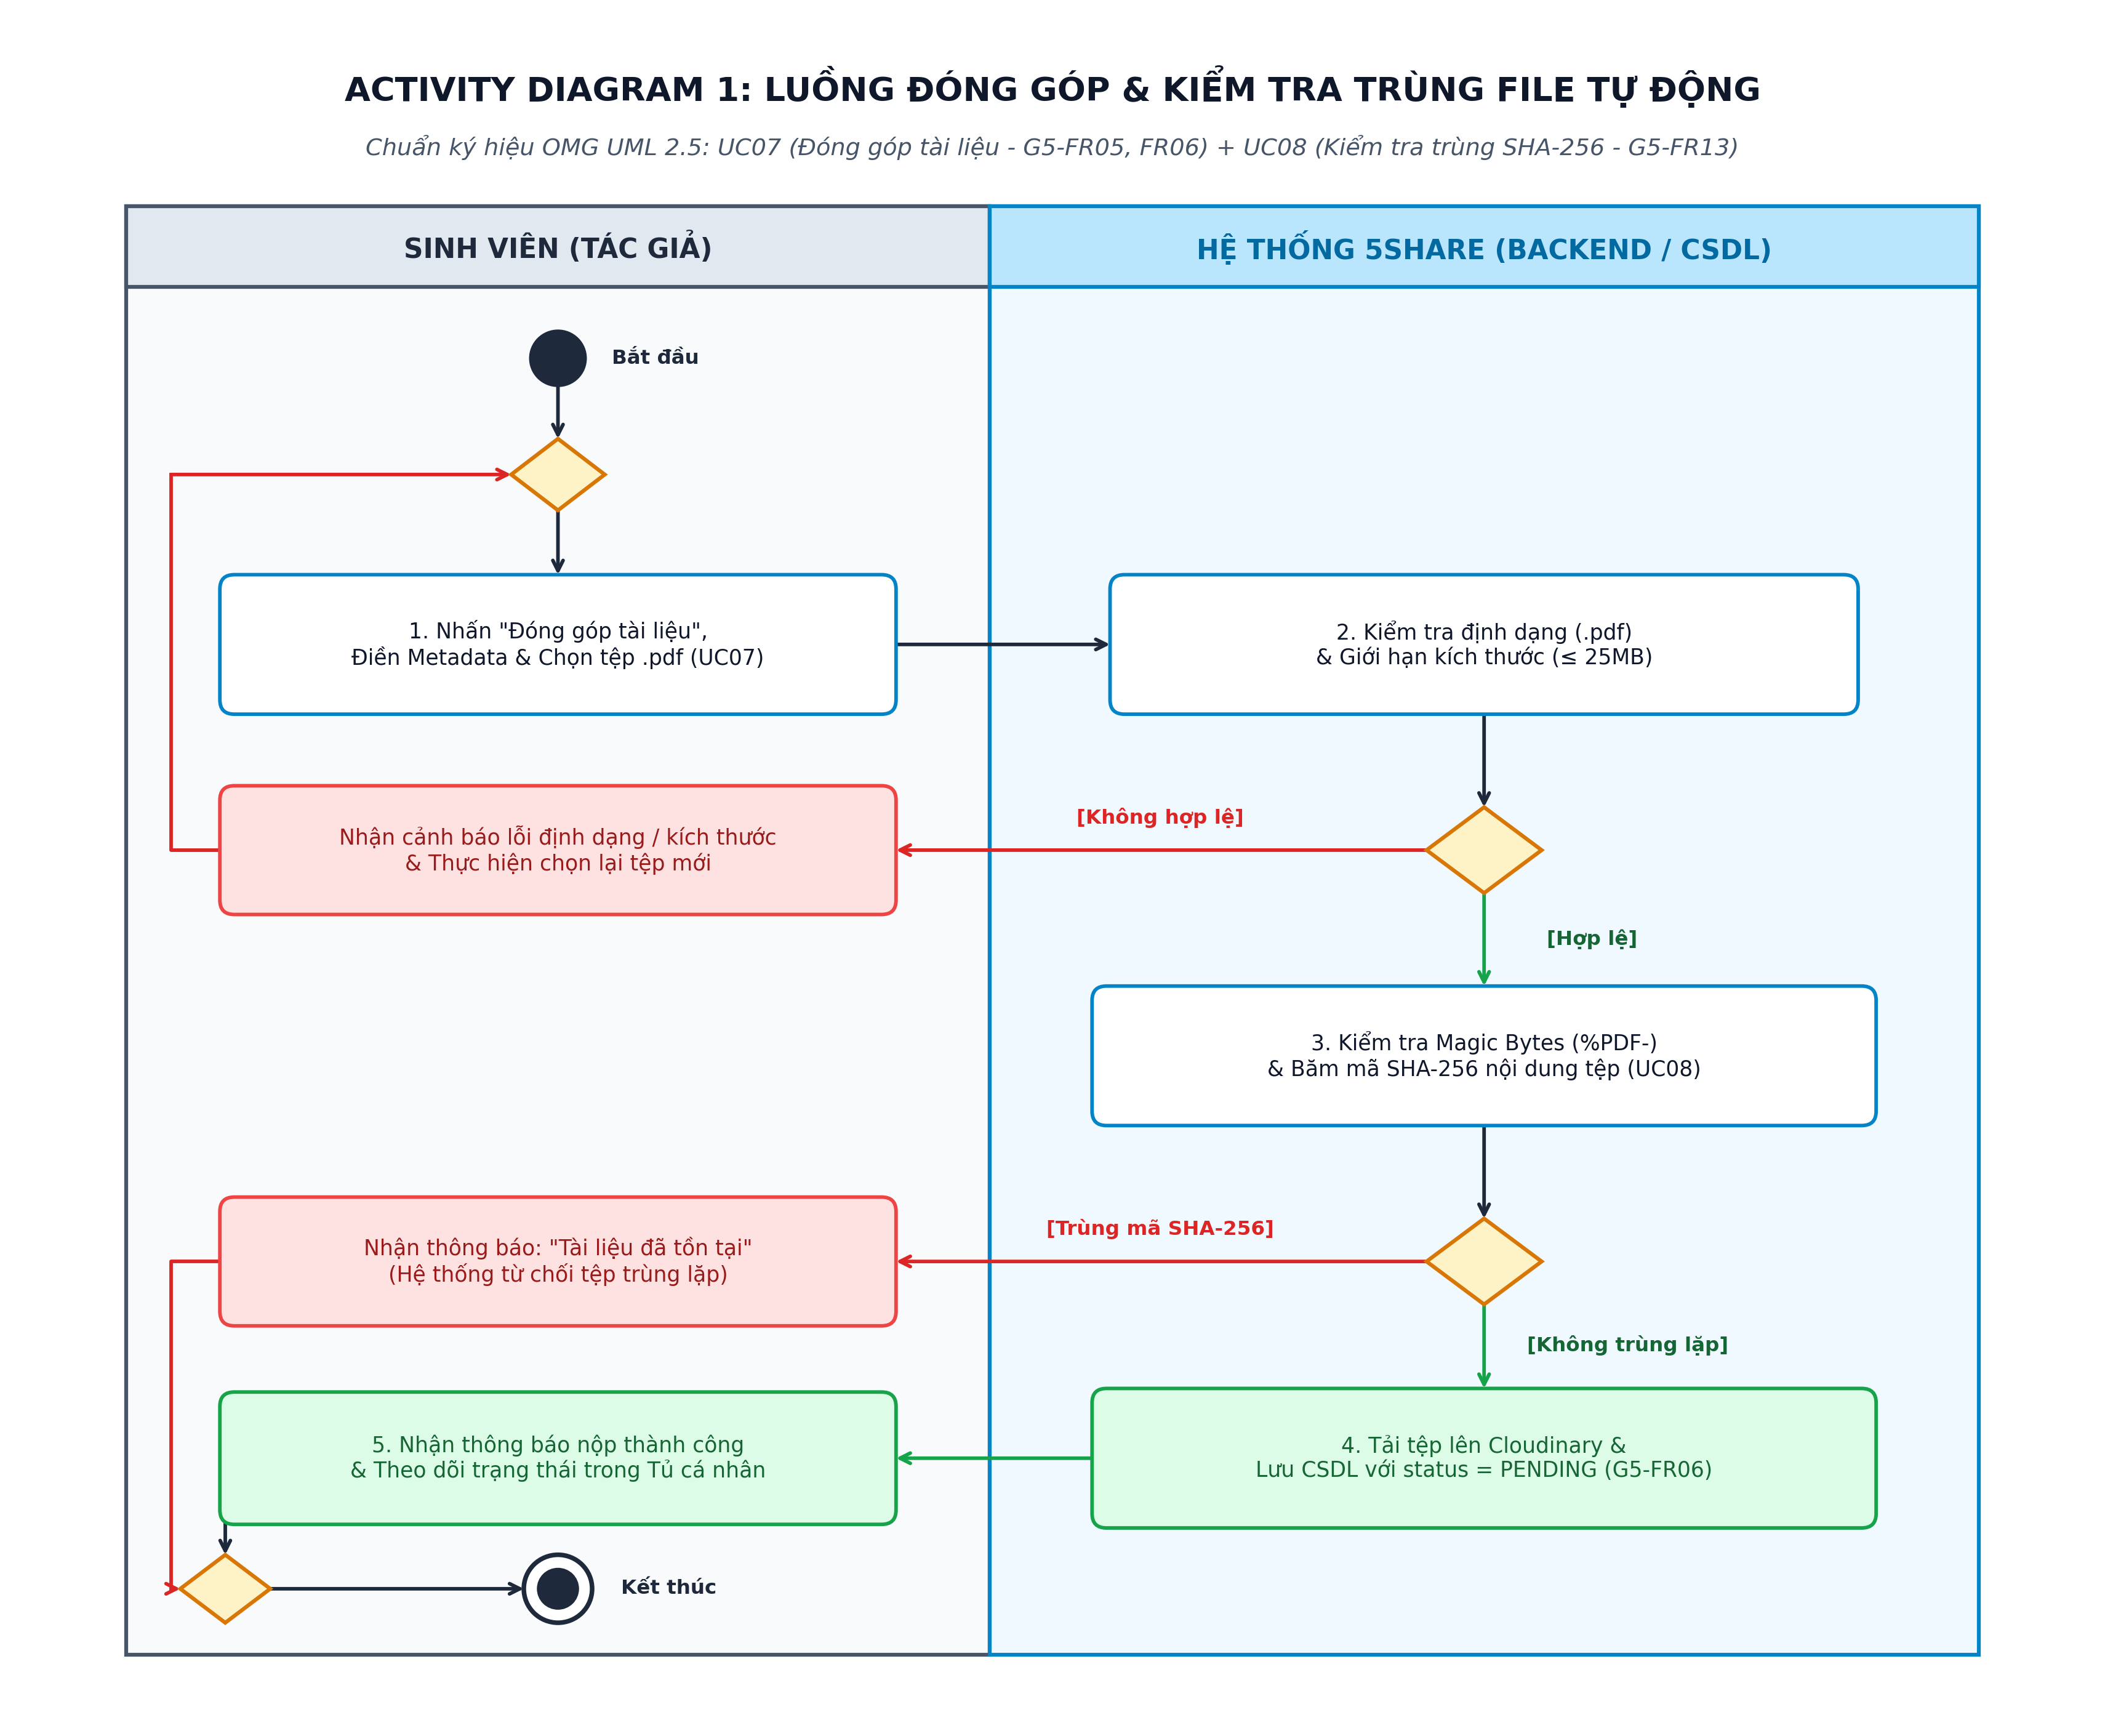
\includegraphics[width=0.96\textwidth]{chuong2/images/ad1_dong_gop_kiem_tra_trung.png}%
}{%
    \fbox{\parbox{0.95\textwidth}{\centering \vspace{3cm}\textbf{[Hình 2.3: Biểu đồ hoạt động luồng đóng góp và kiểm tra trùng lặp tự động (AD1)]}\vspace{3cm}}}%
}
\caption{Biểu đồ hoạt động luồng đóng góp và kiểm tra trùng lặp tự động (AD1)}
\label{fig:ad1}
\end{figure}

Quy trình kiểm soát tự động trên biểu đồ diễn ra theo 3 chốt chặn kỹ thuật liên tiếp:
\begin{itemize}[leftmargin=*,noitemsep]
    \item \textbf{Chốt chặn 1 -- Kiểm tra biểu mẫu Metadata:} Sau khi sinh viên chọn tệp PDF và nhập đầy đủ các trường Metadata bắt buộc (Tên tài liệu, Môn học, Loại học liệu, Mô tả), hệ thống kiểm tra tính hợp lệ của biểu mẫu. Nếu thiếu thông tin, luồng điều khiển đi qua nút gộp (\textit{Merge Node}) quay lại bước nhập liệu để sinh viên bổ sung.
    \item \textbf{Chốt chặn 2 -- Kiểm tra định dạng và dung lượng:} Hệ thống kiểm tra định dạng tệp (\texttt{.pdf}), chữ ký nhị phân đầu tệp (Magic Bytes \texttt{\%PDF-}) và giới hạn dung lượng $\le$ 25MB. Nếu tệp tin vượt quá dung lượng hoặc giả mạo định dạng, hệ thống cảnh báo lỗi và yêu cầu chọn lại tệp.
    \item \textbf{Chốt chặn 3 -- Băm SHA-256 chống trùng lặp:} Hệ thống kích hoạt thuật toán băm \texttt{SHA-256} trên nội dung nhị phân của tệp tin (\texttt{UC08}) và đối chiếu với cột \texttt{file\_hash} trong bảng \texttt{documents}. Nếu mã băm đã tồn tại, hệ thống từ chối tiếp nhận và kết thúc luồng tại nút kết thúc (\textit{Activity Final Node}). Nếu mã băm là duy nhất, hệ thống tải tệp lên dịch vụ đám mây Cloudinary, khởi tạo bản ghi với trạng thái \texttt{status = 'PENDING'} và chuyển sang màn hình theo dõi trạng thái tài liệu (\texttt{UC11}).
\end{itemize}

\subsubsection{2.4.2. Biểu đồ hoạt động luồng tra cứu, xem trước và tải học liệu}
Biểu đồ hoạt động thứ hai (Hình~\ref{fig:ad2}) mô tả luồng nghiệp vụ kết hợp giữa các ca sử dụng \texttt{UC05} (Tìm kiếm và lọc tài liệu), \texttt{UC06} (Xem trước tài liệu), \texttt{UC12} (Tải tài liệu về máy) và \texttt{UC01} (Đăng nhập hệ thống) giữa 02 làn bơi: Người dùng (Khách vãng lai / Sinh viên) và Hệ thống 5Share.

\begin{figure}[H]
\centering
\IfFileExists{chuong2/images/ad2_tra_cuu_preview_tai_ve.png}{%
    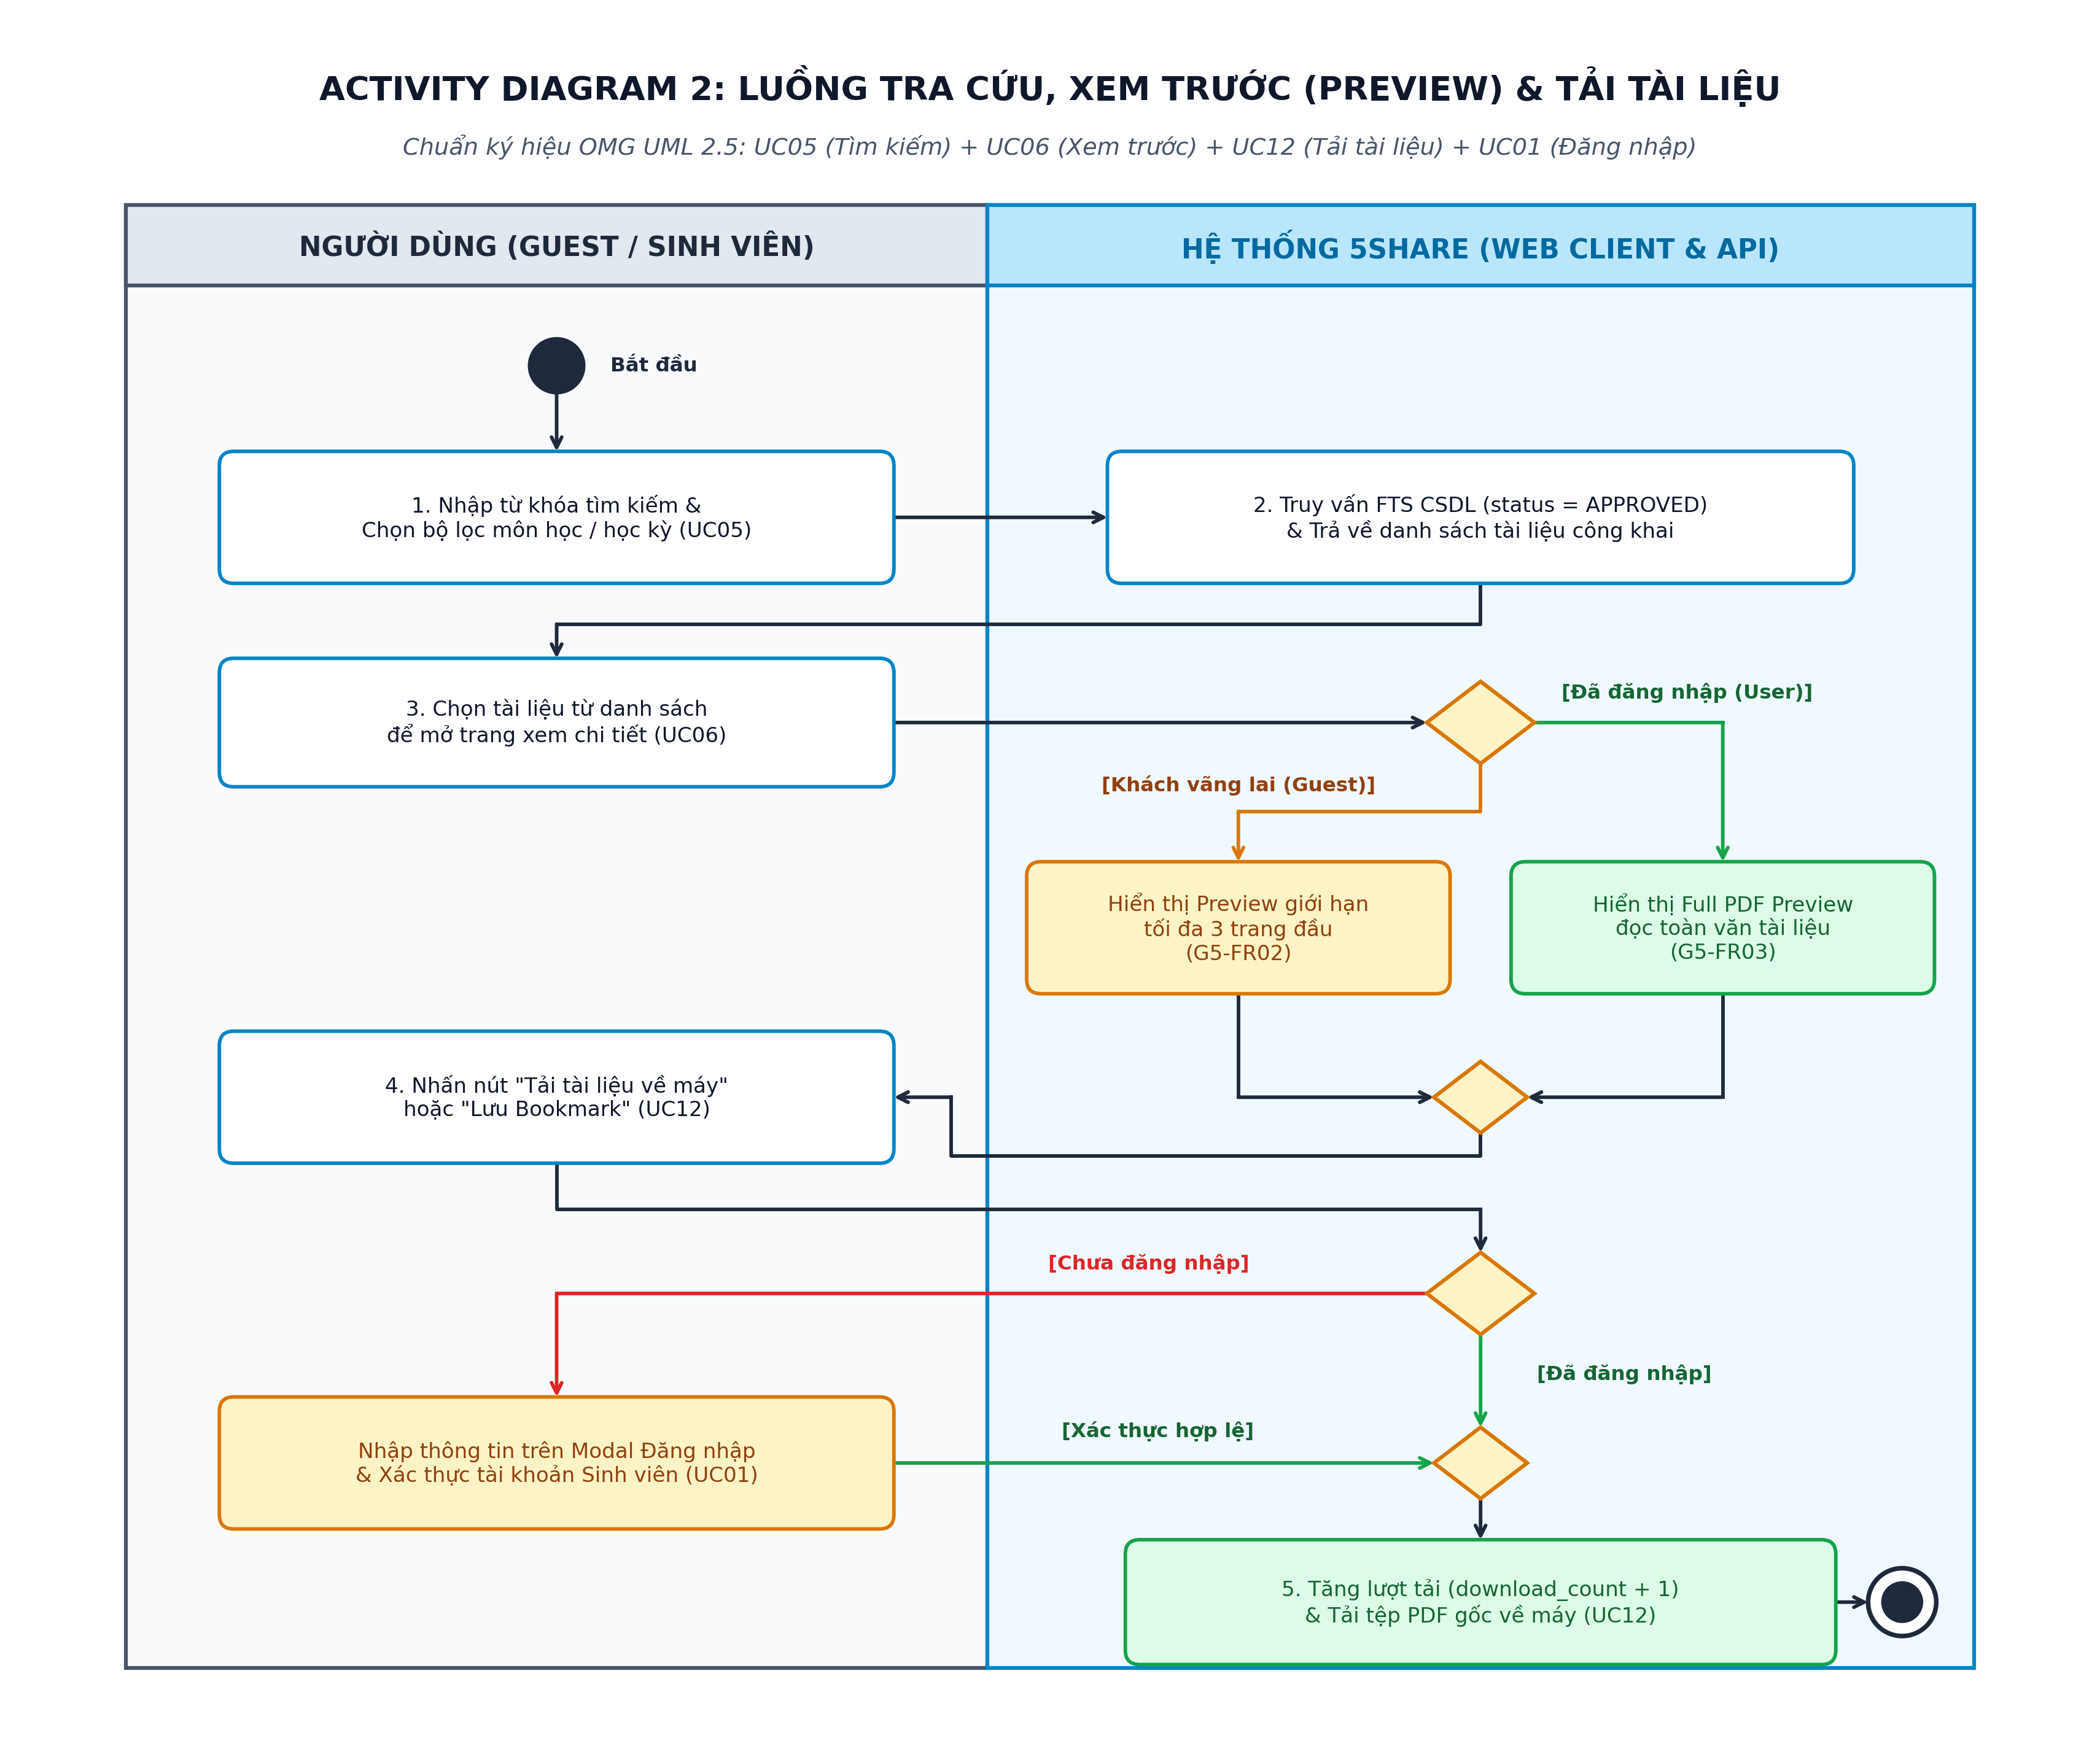
\includegraphics[width=0.96\textwidth]{chuong2/images/ad2_tra_cuu_preview_tai_ve.png}%
}{%
    \fbox{\parbox{0.95\textwidth}{\centering \vspace{3cm}\textbf{[Hình 2.4: Biểu đồ hoạt động luồng tra cứu, xem trước và tải học liệu (AD2)]}\vspace{3cm}}}%
}
\caption{Biểu đồ hoạt động luồng tra cứu, xem trước và tải học liệu (AD2)}
\label{fig:ad2}
\end{figure}

Luồng hoạt động thể hiện rõ cơ chế phân quyền truy cập tài nguyên theo trạng thái xác thực:
\begin{itemize}[leftmargin=*,noitemsep]
    \item \textbf{Giai đoạn tra cứu và lọc:} Người dùng nhập từ khóa hoặc chọn bộ lọc theo môn học, loại học liệu. Hệ thống truy vấn cơ sở dữ liệu bằng Full-Text Search đối với các bản ghi có \texttt{status = 'APPROVED'}. Nếu không có kết quả khớp, hệ thống thông báo để người dùng điều chỉnh từ khóa.
    \item \textbf{Giai đoạn xem trước trực tuyến (Preview):} Khi người dùng chọn một học liệu, hệ thống hiển thị bản xem trước trực tuyến trên trình duyệt (\texttt{UC06}). Khách vãng lai được đọc thử tối đa 3 trang đầu tiên; nếu chỉ dừng lại ở việc xem thử và đóng trang, luồng hoạt động kết thúc bình thường.
    \item \textbf{Giai đoạn kiểm tra phiên đăng nhập và tải tệp gốc:} Khi người dùng nhấn nút ``Tải xuống tệp gốc (.pdf)'' (\texttt{UC12}), hệ thống kiểm tra mã phiên xác thực JWT. Nếu người dùng đã đăng nhập, hệ thống tăng bộ đếm \texttt{download\_count} thêm 1 và trả luồng tệp PDF gốc về thiết bị. Nếu người dùng là Khách vãng lai, hệ thống mở cửa sổ yêu cầu đăng nhập (\texttt{UC01}); ngay sau khi xác thực thành công, luồng điều khiển hợp nhất tại nút Merge để tự động thực thi việc tải tệp mà không bắt người dùng phải tìm kiếm lại từ đầu.
\end{itemize}

\subsubsection{2.4.3. Biểu đồ quy trình nghiệp vụ (BPMN 2.0) vòng đời kiểm duyệt và khai thác học liệu}
Để mô tả toàn diện sự phối hợp liên tác nhân xuyên suốt vòng đời của một học liệu số từ lúc sinh viên đóng góp, trải qua kiểm duyệt hai tầng cho đến khi xuất bản công khai hoặc bị thu hồi do vi phạm, biểu đồ quy trình nghiệp vụ cộng tác theo chuẩn OMG BPMN 2.0 gồm 03 bể (\textit{Pools}) độc lập được xây dựng tại Hình~\ref{fig:bpmn_vong_doi}:

\begin{figure}[H]
\centering
\IfFileExists{chuong2/images/bpmn_vong_doi_tai_lieu.png}{%
    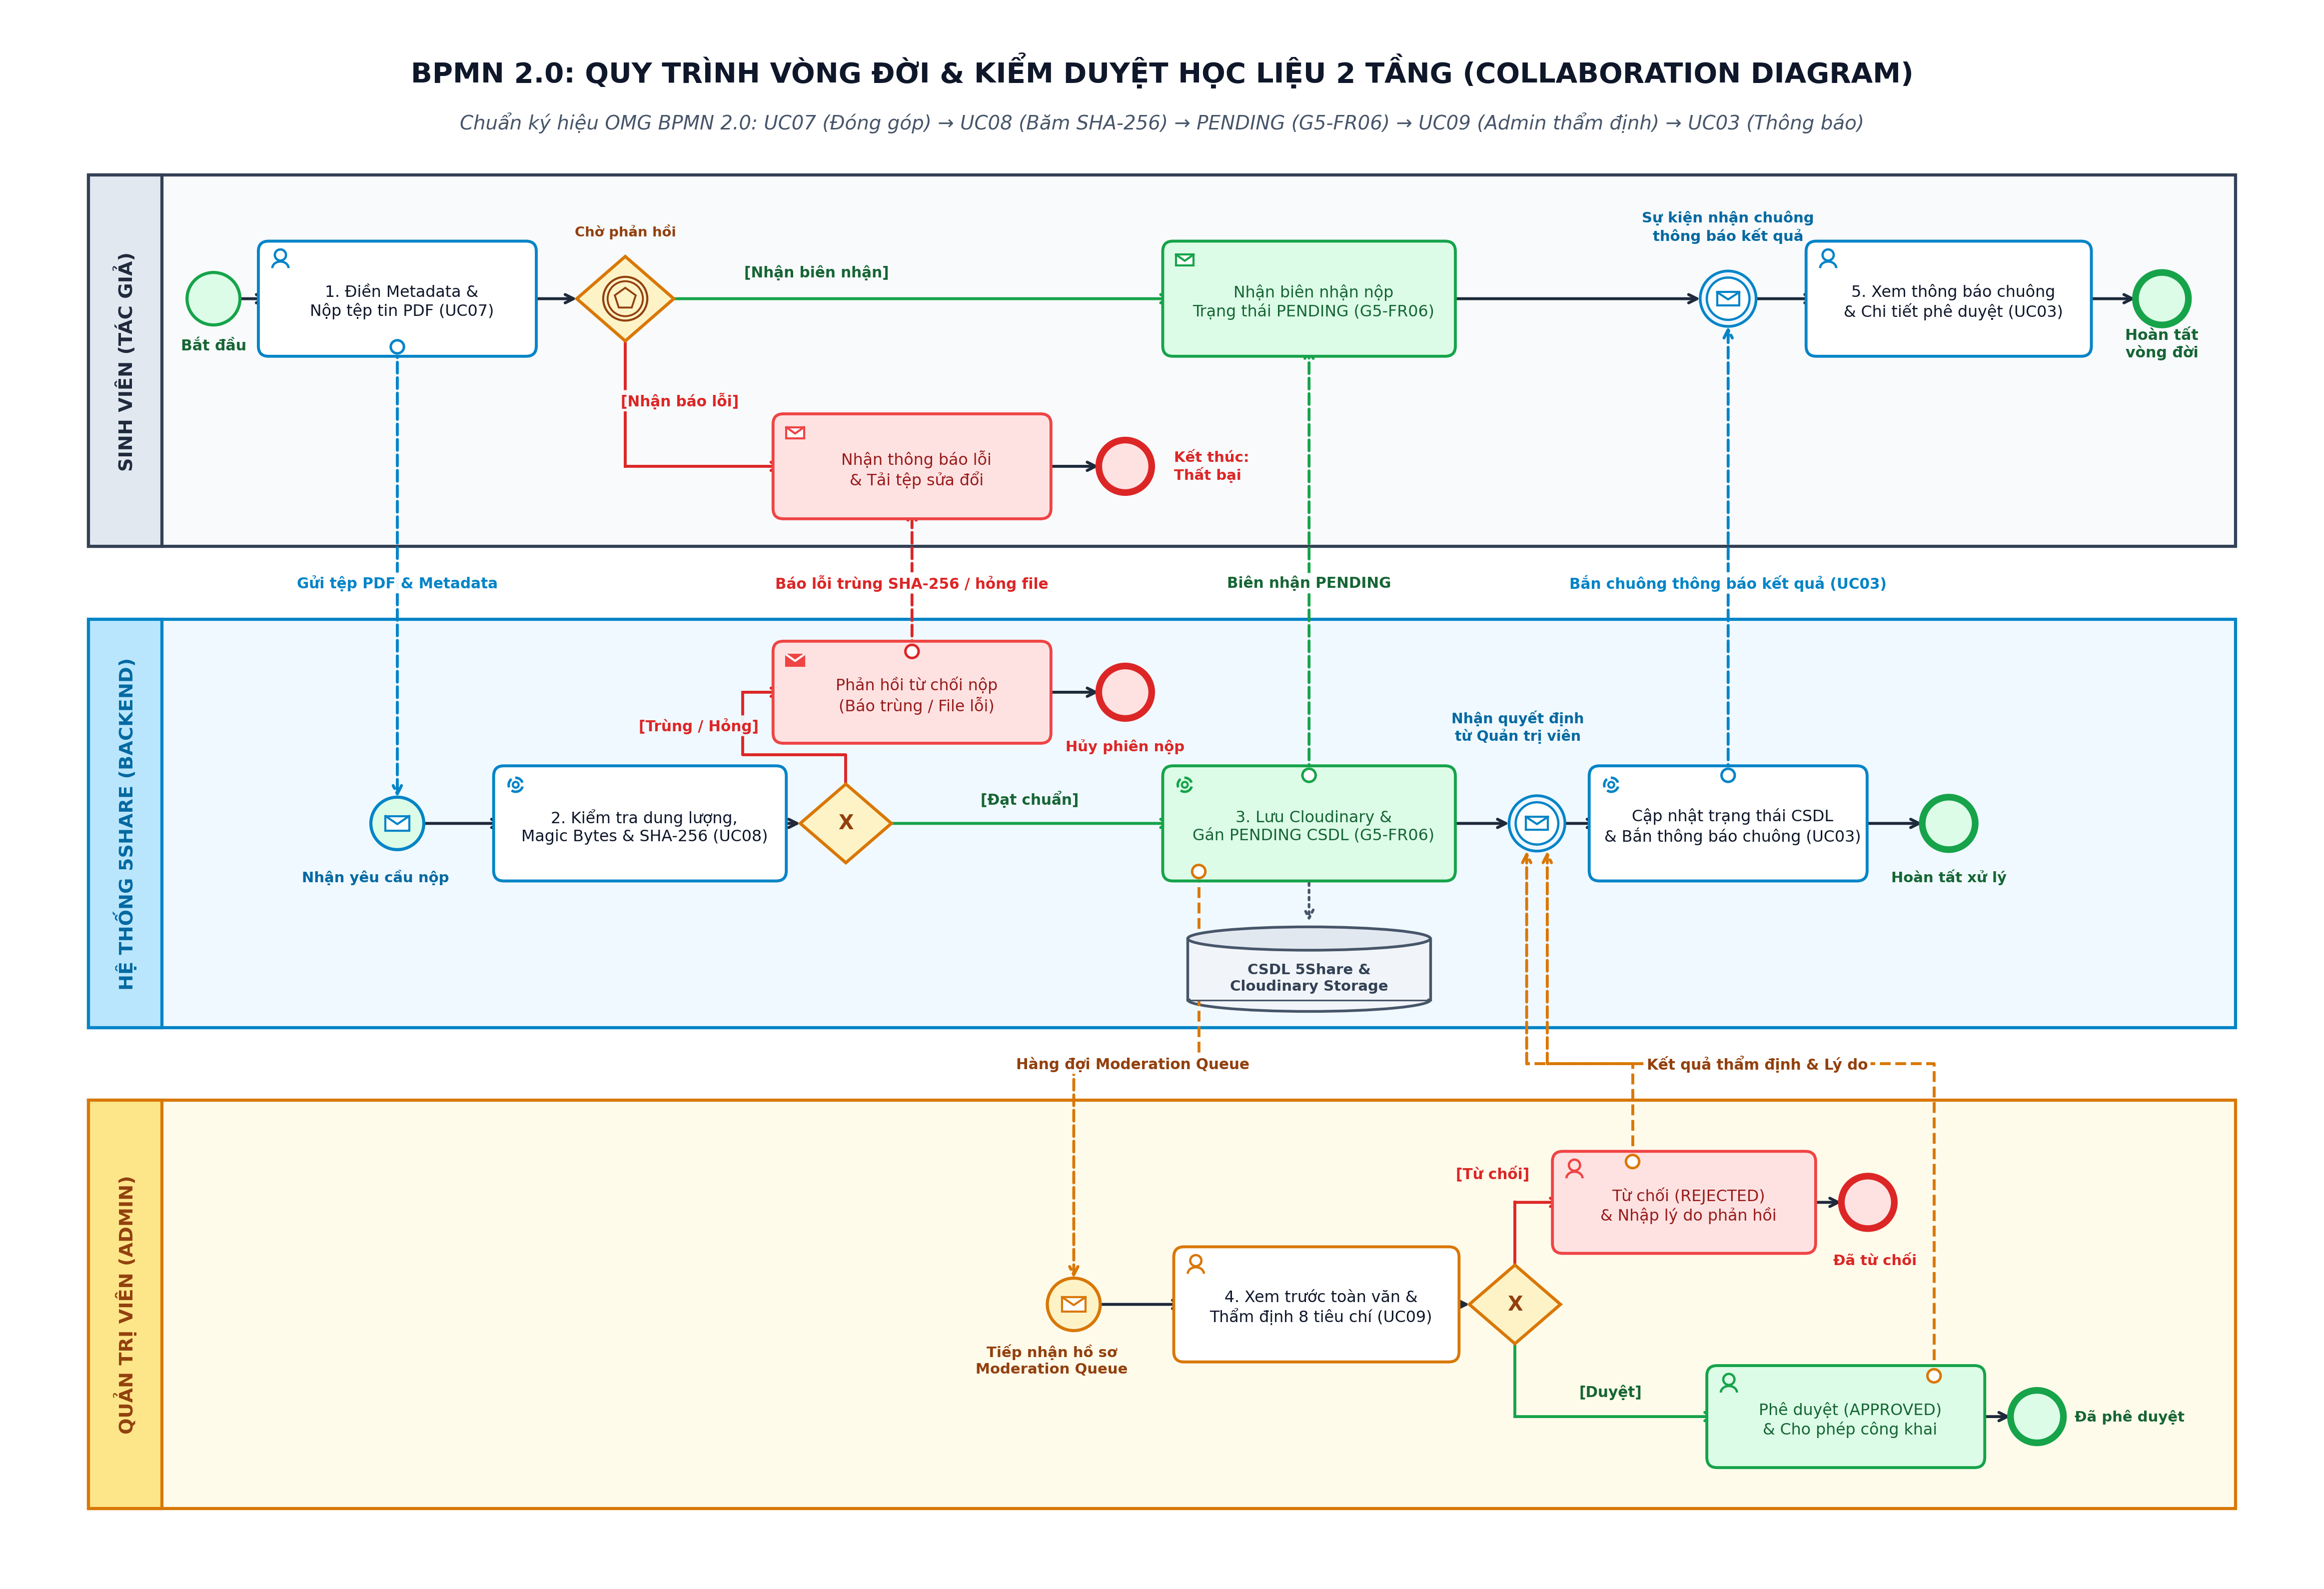
\includegraphics[width=0.99\textwidth]{chuong2/images/bpmn_vong_doi_tai_lieu.png}%
}{%
    \fbox{\parbox{0.95\textwidth}{\centering \vspace{3cm}\textbf{[Hình 2.5: Biểu đồ quy trình nghiệp vụ (BPMN 2.0) vòng đời kiểm duyệt và khai thác học liệu trên 5Share]}\vspace{3cm}}}%
}
\caption{Biểu đồ quy trình nghiệp vụ (BPMN 2.0) vòng đời kiểm duyệt và khai thác học liệu trên 5Share}
\label{fig:bpmn_vong_doi}
\end{figure}

Cấu trúc biểu đồ tuân thủ nghiêm ngặt các nguyên tắc ký hiệu của chuẩn OMG BPMN 2.0:
\begin{itemize}[leftmargin=*,noitemsep]
    \item \textbf{Phân tách bể (Pools) và làn (Lanes):} Biểu đồ phân tách rõ 03 Pool đại diện cho 3 chủ thể: (1) Pool Sinh viên (Tác giả đóng góp \& Người học khai thác); (2) Pool Hệ thống 5Share (chứa 2 làn nội bộ: Làn Kiểm tra tự động \& Xử lý sự kiện, và Làn Lưu trữ đám mây \& Cơ sở dữ liệu); (3) Pool Quản trị viên (Ban kiểm duyệt học liệu).
    \item \textbf{Luồng tuần tự (Sequence Flow) và Luồng thông điệp (Message Flow):} Mọi tương tác bên trong cùng một Pool được nối bằng mũi tên nét liền (\textit{Sequence Flow}). Mọi tương tác vượt qua ranh giới giữa hai Pool khác nhau bắt buộc sử dụng đường nét đứt có vòng tròn ở gốc (\textit{Message Flow}), kết nối từ các tác vụ gửi (\textit{Send Task}) hoặc tác vụ dịch vụ (\textit{Service Task}) đến các sự kiện bắt thông điệp (\textit{Message Start/Intermediate Catch Event}).
    \item \textbf{Cổng hướng sự kiện (Event-Based Gateway) và Vòng đời hậu kiểm:} Sau khi gửi biểu mẫu đóng góp (\texttt{UC07}), luồng của Sinh viên đi vào cổng rẽ nhánh dựa trên sự kiện (\textit{Event-Based Gateway}) để chờ phản hồi từ hệ thống qua 3 nhánh sự kiện bắt thông điệp: (1) Nhận cảnh báo lỗi kỹ thuật hoặc trùng mã băm \texttt{SHA-256} (từ \texttt{UC08}); (2) Nhận thông báo tài liệu bị từ chối kèm lý do (\texttt{REJECTED}); (3) Nhận thông báo tài liệu được phê duyệt (\texttt{APPROVED}) và cộng điểm đóng góp. Đối với tài liệu đã xuất bản, nếu bị sinh viên khác gửi báo cáo vi phạm (\texttt{UC04}) và Quản trị viên xác nhận vi phạm nặng (\texttt{UC09}), hệ thống thực thi tác vụ thu hồi (\texttt{status = 'HIDDEN'} / \texttt{'DELETED'}) để bảo đảm độ tinh sạch của kho học liệu.
\end{itemize}

\newpage
\subsection{2.5. Đặc tả các yêu cầu phi chức năng}
Bên cạnh 13 yêu cầu chức năng cốt lõi, hệ thống 5Share phải đáp ứng các yêu cầu phi chức năng (\textit{Non-Functional Requirements}) nhằm bảo đảm tính dễ sử dụng, hiệu năng phản hồi, an toàn bảo mật và độ tin cậy trong vận hành thực tế.

\subsubsection{2.5.1. Yêu cầu về tính dễ sử dụng và giao diện}
\begin{itemize}[leftmargin=*,noitemsep]
    \item \textbf{Tương thích đa thiết bị:} Giao diện người dùng được thiết kế theo hướng thích ứng đa thiết bị (\textit{Responsive Web Design}), hiển thị chuẩn xác trên cả màn hình máy tính để bàn, máy tính xách tay và thiết bị di động của sinh viên.
    \item \textbf{Trải nghiệm đọc trực tuyến liền mạch:} Tích hợp trình đọc PDF trực tiếp trên nền tảng web có hỗ trợ bộ ký tự Unicode tiếng Việt (CMAP), cho phép sinh viên xem ngay nội dung Kế hoạch bài dạy 5512, đề thi và bài giảng mà không cần cài đặt phần mềm bên thứ ba.
    \item \textbf{Thông điệp phản hồi trực quan:} Mọi thông báo lỗi xác thực, cảnh báo vượt dung lượng, cảnh báo trùng lặp tệp tin và lý do từ chối kiểm duyệt đều được hiển thị bằng tiếng Việt rõ ràng, lịch sự và hướng dẫn cụ thể cách khắc phục.
\end{itemize}

\subsubsection{2.5.2. Yêu cầu về hiệu năng và tốc độ phản hồi}
\begin{itemize}[leftmargin=*,noitemsep]
    \item \textbf{Tốc độ xác thực phiên làm việc:} Thời gian xử lý yêu cầu đăng nhập, kiểm tra mã phiên JWT và phản hồi điều hướng giao diện đạt dưới 1 giây trong điều kiện mạng tiêu chuẩn.
    \item \textbf{Hiệu năng tìm kiếm và lọc học liệu:} Các truy vấn tìm kiếm toàn văn (Full-Text Search) kết hợp lọc theo môn học, học kỳ và phân trang (12 tài liệu/trang) trả kết quả trong thời gian dưới 2 giây.
    \item \textbf{Tốc độ hiển thị bản xem trước và kiểm tra mã băm:} Thời gian tải và hiển thị 3 trang đầu tiên của tài liệu PDF trên trình duyệt đạt dưới 2,5 giây; thuật toán tính mã băm \texttt{SHA-256} và đối chiếu chỉ mục chống trùng lặp cho tệp tin 25MB hoàn tất trong vòng 500ms ở tầng máy chủ.
\end{itemize}

\subsubsection{2.5.3. Yêu cầu về an toàn và bảo mật dữ liệu}
\begin{itemize}[leftmargin=*,noitemsep]
    \item \textbf{Bảo mật thông tin xác thực:} Toàn bộ mật khẩu tài khoản người dùng bắt buộc phải được băm một chiều bằng thuật toán \texttt{bcrypt} trước khi lưu xuống cơ sở dữ liệu; sử dụng chuẩn JSON Web Token (JWT) có thời hạn để xác thực các yêu cầu gọi API.
    \item \textbf{Kiểm soát phân quyền truy cập (RBAC):} Áp dụng cơ chế phân quyền dựa trên vai trò (\textit{Role-Based Access Control -- RBAC}) gồm 3 mức: Khách vãng lai, Sinh viên và Quản trị viên. Tài khoản Quản trị viên được cố định và bảo vệ ở tầng cơ sở dữ liệu; người dùng thông thường không thể tự nâng quyền.
    \item \textbf{An toàn tệp tin đầu vào:} Mọi tệp tin tải lên đều phải vượt qua bước kiểm tra chữ ký nhị phân đầu tệp (Magic Bytes phải khớp chuỗi \texttt{\%PDF-}) và giới hạn dung lượng $\le$ 25MB nhằm ngăn chặn tuyệt đối hành vi đổi đuôi tệp thực thi độc hại (\texttt{.exe}, \texttt{.sh}, \texttt{.bat}) thành \texttt{.pdf}.
    \item \textbf{Bảo vệ tài nguyên học liệu:} Các tài liệu đang ở trạng thái chờ duyệt (\texttt{status = 'PENDING'}) hoặc bị từ chối (\texttt{status = 'REJECTED'}) bị khóa truy cập công khai ở tầng API; Khách vãng lai bị chặn truy xuất đường dẫn tải tệp gốc trên đám mây khi chưa xác thực.
\end{itemize}

\subsubsection{2.5.4. Yêu cầu về tính ổn định và ràng buộc thiết kế}
\begin{itemize}[leftmargin=*,noitemsep]
    \item \textbf{Kiến trúc lưu trữ phân tách:} Hệ thống tách biệt tầng lưu trữ dữ liệu có cấu trúc (cơ sở dữ liệu quan hệ PostgreSQL) và tầng lưu trữ tệp tin vật lý (dịch vụ đám mây Cloudinary), giúp máy chủ ứng dụng không bị quá tải dung lượng đĩa cứng khi số lượng học liệu tăng lên.
    \item \textbf{Toàn vẹn dữ liệu:} Áp dụng ràng buộc khóa ngoại (\textit{Foreign Key}) và cơ chế giao dịch (\textit{Transaction}) trong cơ sở dữ liệu; đối với các môn học đã có tài liệu liên kết, hệ thống chỉ cho phép chuyển trạng thái ẩn/vô hiệu hóa thay vì xóa vật lý nhằm bảo toàn lịch sử học liệu.
\end{itemize}

Các chỉ số yêu cầu phi chức năng trọng tâm của hệ thống 5Share được tổng hợp định lượng tại Bảng~\ref{tab:nfr_summary}:

\begin{table}[H]
\centering
\footnotesize\linespread{1.05}\selectfont
\setlength{\tabcolsep}{5pt}
\renewcommand{\arraystretch}{1.12}
\begin{tabularx}{\textwidth}{|c|p{3.6cm}|X|p{2.8cm}|}
\hline
\rowcolor[HTML]{EAEAEA}
\textbf{STT} & \textbf{Nhóm yêu cầu phi chức năng} & \textbf{Chỉ số kỹ thuật / Ràng buộc áp dụng} & \textbf{Ca sử dụng liên quan} \\
\hline
1 & Hiệu năng xác thực và thông báo & Thời gian phản hồi đăng nhập JWT $<$ 1 giây; thời gian tải danh sách thông báo chuông $<$ 500ms. & \texttt{UC01}, \texttt{UC02}, \texttt{UC03} \\
\hline
2 & Hiệu năng tra cứu và xem trước PDF & Tìm kiếm Full-Text Search tiếng Việt và lọc đa tiêu chí $<$ 2 giây (phân trang 12 tài liệu/trang); hiển thị 3 trang xem thử đầu tiên $<$ 2,5 giây. & \texttt{UC05}, \texttt{UC06} \\
\hline
3 & Hiệu năng chống trùng lặp tệp tin & Tính toán mã băm \texttt{SHA-256} (64 ký tự hex) từ luồng nhị phân và đối chiếu cột \texttt{file\_hash} $<$ 500ms cho tệp tối đa 25MB. & \texttt{UC07}, \texttt{UC08} \\
\hline
4 & An toàn tệp tin và Lưu trữ đám mây & Bắt buộc định dạng \texttt{.pdf}, dung lượng $\le$ 25MB, kiểm tra chữ ký nhị phân Magic Bytes \texttt{\%PDF-}; lưu trữ tệp vật lý tách biệt trên Cloudinary. & \texttt{UC07}, \texttt{UC12} \\
\hline
5 & Bảo mật mật khẩu và Phân quyền RBAC & Mã hóa mật khẩu bằng thuật toán \texttt{bcrypt}; kiểm soát truy cập API theo vai trò (Guest / Student / Admin); ẩn tuyệt đối tài liệu \texttt{PENDING} khỏi kho công khai. & \texttt{UC01}, \texttt{UC02}, \texttt{UC06}, \texttt{UC09}, \texttt{UC11}, \texttt{UC12} \\
\hline
6 & Toàn vẹn dữ liệu và Chống lặp tương tác & Mỗi tài khoản chỉ chấm sao 1 lần/tài liệu; chặn gửi báo cáo vi phạm trùng lặp; cấm xóa cứng môn học đang chứa tài liệu. & \texttt{UC04}, \texttt{UC10}, \texttt{UC13} \\
\hline
\end{tabularx}
\caption{Tổng hợp các chỉ số yêu cầu phi chức năng của hệ thống 5Share}
\label{tab:nfr_summary}
\end{table}

